%%% use twocolumn and 10pt options with the asme2ej format
\documentclass[10pt]{asme2ej}
%\usepackage{epstopdf}
\usepackage{epsfig} %% for loading postscript figures
\usepackage{graphicx}
\usepackage{epstopdf}
\usepackage{float}
\usepackage{amsmath}
\usepackage{subcaption}
\usepackage{stfloats}
\usepackage{threeparttable}
\usepackage{fancyhdr}

\pagestyle{fancy}
\renewcommand{\headrulewidth}{0pt}
\fancyhf{}
\lfoot{JMR-19-1300}
\cfoot{Fu}
\rfoot{\thepage}

\usepackage{array}
\usepackage{algorithmic}
\usepackage{algorithm}
\usepackage{multirow}
\usepackage{rotating}
\usepackage{mathrsfs}
\usepackage{color}
\usepackage[normalem]{ulem}
\usepackage{wasysym}
%\usepackage{multirow}
% for figures: caption label is italic, the caption text is bold / italic

\graphicspath{,{./figs/}}

% \linespread{2}
%% The class has several options
%  onecolumn/twocolumn - format for one or two columns per page
%  10pt/11pt/12pt - use 10, 11, or 12 point font
%  oneside/twoside - format for oneside/twosided printing
%  final/draft - format for final/draft copy
%  cleanfoot - take out copyright info in footer leave page number
%  cleanhead - take out the conference banner on the title page
%  titlepage/notitlepage - put in titlepage or leave out titlepage
%  
%% The default is oneside, onecolumn, 10pt, final

\title{A Lower Limb Exoskeleton Recycling Energy from Knee and Ankle Joints to Assist Push-Off}

%%% first author
\author{Yihua Chang$^\ast$
	\affiliation{
		State Key Laboratory of Tribology\\
		Tsinghua University\\
		Beijing, China, 100084\\
		Email: changyh16@mails.tsinghua.edu.cn
	}	
}

\author{Weixin Wang\thanks{These two authors contributed equally to this work.}
	\affiliation{
		State Key Laboratory of Tribology\\
		Tsinghua University\\
		Beijing, China, 100084\\
		Email: weixinwang442@gmail.com
	}	
}

\author{Chenglong Fu\thanks{Corresponding author.}
    \affiliation{ 
    Department of Mechanical and Energy Engineering\\
	Southern University of Science and Technology\\
	Shenzhen, China, 518055\\
	Email:  fucl@sustech.edu.cn
    }
}

\begin{document}

\maketitle    

%%%%%%%%%%%%%%%%%%%%%%%%%%%%%%%%%%%%%%%%%%%%%%%%%%%%%%%%%%%%%%%%%%%%%%
\begin{abstract}
{\it This paper presents the design and preliminary evaluation of a quasi-passive lower limb exoskeleton for walking efficiency improvements.
The exoskeleton recycles the negative work performed by the knee joint in late swing phase and the ankle joint in mid-stance phase, to assist ankle push-off in late stance phase when a burst of positive power is needed.
The exoskeleton consists of a torsion spring as an energy storage element, and two clutches attached to both ends of the spring to control the timing of recycling and releasing energy in a gait cycle.
The two clutches are actively controlled by two small servo motors with very low power consumption based on the plantar pressure.
The novelty of this exoskeleton is it makes the extra kinetic energy dissipated at the knee joint reusable, by transferring it to the ankle joint to assist positive power generation during push-off, for the first time.
Eight male subjects walked with the exoskeleton engaged (EXO\_ON), disengaged (EXO\_OFF) and without the exoskeleton (NO\_EXO).
Inverse dynamics analysis demonstrated reduced negative biological work at the knee joint during late swing and at the ankle joint during mid stance, as well as reduced positive biological work at the ankle joint during late stance comparing the EXO\_ON to EXO\_OFF conditions.
These results prove the effectiveness of the exoskeleton at joint level.
	
Keywords: human walking, quasi-passive exoskeleton, energy recycling, clutch-spring, joint power}

\end{abstract}

%%%%%%%%%%%%%%%%%%%%%%%%%%%%%%%%%%%%%%%%%%%%%%%%%%%%%%%%%%%%%%%%%%%%%%

%%%%%%%%%%%%%%%%%%%%%%%%%%%%%%%%%%%%%%%%%%%%%%%%%%%%%%%%
%%%                                     
%%%  1. Introduction                    
%%%                                     
%%%%%%%%%%%%%%%%%%%%%%%%%%%%%%%%%%%%%%%%%%%%%%%%%%%%%%%%
\section{Introduction}       
\label{sec:intro}

Humans consume more energy during walking than any other activities in daily life.
For a long time, researchers have been attempting to develop lower limb exoskeletons to assist walking.
However, the excessive amount of power required at lower limb joints during walking leads to undesirable sizes and weights of actuators\cite{RN1}.
For instance, the peak value of the ankle joint power during late stance plantar flexion is about 270W for a 70kg person\cite{RN2}.
Therefore, designers have to make a trade-off between the assisting capability and portability.
To circumvent this dilemma, passive/quasi-passive exoskeletons were proposed\cite{RN3}.
These exoskeletons do not directly provide external energy to the human user.
Instead, they use some smart mechanical structures to recycle the dissipated energy during decelerating segments in walking, and supply this recycled energy when positive power is required.

These (quasi-)passive exoskeletons typically use passive elements, mostly dampers and springs, instead of powerful actuators to apply torques at lower limb joints.
The damper is a pure energy absorbing element to dissipate excessive kinetic energy during locomotion, which would otherwise cost extra physiological energy\cite{negativework}.
The exoskeleton built by Walsh \emph{et al.} uses a magnetorheological damper to help the knee joint produce negative work during normal walking\cite{RN3}.

The spring in theory does not produce or dissipate energy, but its ability to store and return energy makes it a good candidate to interact with human limbs. 
Energy storage and return is also a strategy utilized by humans to make locomotion more energetically efficient.
It has been shown the muscle-tendon unit can serve as an energy storage element during walking \cite{RN16,pays}.
By replacing tendons with physical springs, mechanical fixations can be used to replace muscles to produce the counteracting force while the tendon is being stretched.
Exoskeletons described in \cite{RN3,RN4,RN5} use springs spanning hip joints and ankle joints, or only ankle joints to help the respective muscle-tendon units store and return energy.
In addition, springs are also used to shape the biological leg stiffness during stance phase in running, or in other words, decrease the large load exerted at lower limb joints after heel strike \cite{RN6,RN7,RN8}.

Among these exoskeletons, using external moments to assist late stance ankle plantar flexion has been well proved to benefit human walking \cite{RN5,RN9,RN10,RN11,RN12,liu2019ankle}.
The exoskeleton built by Collins \emph{et al.}\cite{RN5} uses a spring to assist the Achilles tendon to store energy in dorsiflexion during stance phase, and supplies the energy to assist the following ankle plantar flexion, which successfully reduces the metabolic expenditure during walking.
In another work \cite{zhang2017human}, the authors even further reduced the walking metabolic expenditure by applying an optimized assistive torque at ankle, which appears higher than the torque supplied by the quasi-passive exoskeleton in \cite{RN5}.
This may suggest instead of only recycling the passive work from ankle dorsiflexion in stance, it could be more beneficial to have another energy source for ankle assistance.

One potential candidate for such energy source is the knee joint, which absorbs energy in most time of a gait cycle\cite{RN2}.
Therefore it may be beneficial to use a spring instead of the damper in \cite{RN3}, to apply resisting torques at the knee joint and recycle the negative work at the same time.
This part of energy can be regarded as an ‘external’ energy input at the ankle joint, i.e. it may be transferred and used to assist the ankle joint in late stance plantar flexion.
This concept has also been mentioned in some other studies\cite{RN3,RN12}, but no such device has been reported to the best of the authors' knowledge.

In this paper, we present a quasi-passive lower limb exoskeleton which is able to recycle energy from both the extension motion of knee joint in late swing phase, and the dorsiflexion motion of ankle joint in mid-stance phase, to assist the ankle plantar flexion in late stance phase.
The exoskeleton consists of a torsion spring to store energy, and two clutches to control the timing of energy recycling and releasing based on foot contact information.
%In order to evaluate the effectiveness of the exoskeleton, the power of exoskeleton was measured to estimate the amount of energy recycled and released; inverse dynamics analysis was also performed to evaluate the benefits and side-effects to human during walking.
Eight male subjects participated in a study comparing three conditions: walking with the exoskeleton engaged (EXO\_ON), disengaged (EXO\_OFF) and without the exoskeleton (NO\_EXO) on the right leg.
Inverse dynamics analysis showed significant reductions of the biological knee power in late swing phase and ankle power in mid and late stance phase comparing the EXO\_ON to EXO\_Off conditions, suggesting the effectiveness of the exoskeleton at joint level.

The rest of this paper is organized as follows.
In section \ref{sec:design}, we introduce the mechanical and control system design of the proposed exoskeleton.
Then the experiment protocols and results are presented in section \ref{sec:experiment}.
Finally, conclusions and future work are given in section \ref{sec:discussion}.


%%%%%%%%%%%%%%%%%%%%%%%%%%%%%%%%%%%%%%%%%%%%%%%%%%%%%%%%
%%%                                     
%%%  2. Design                 
%%%                                     
%%%%%%%%%%%%%%%%%%%%%%%%%%%%%%%%%%%%%%%%%%%%%%%%%%%%%%%%
\section{Design of the Exoskeleton}
\label{sec:design}

\subsection{Energy Recycling and Releasing Strategies}
\label{subsec:Biomechanics}

Lower limb joints perform both positive and negative work during each gait cycle of human walking, as shown in Fig. \ref{fig:work}.
The stance leg transports the center of mass (COM) of human body along an arched path, which is usually modeled as an inverted pendulum\cite{RN13}.
Before toe off, there is an intensive burst of energy generated at the ankle joint (red solid area, 40-60\% Stride, Fig. \ref{fig:work}).
This part of energy is consumed to redirect the downward velocity of the COM to an upward direction, and initiate the next step as the step-to-step transition \cite{RN14,wu2016effects}.
This process is referred to as push-off, during which the energy dissipated in the collision between the opposite leg and ground is compensated by the positive work generated by the ankle joint.
Push-off consumes nearly 45\% of the metabolic energy expenditure in human walking\cite{RN15}.

\begin{figure}[b]
	\centering
	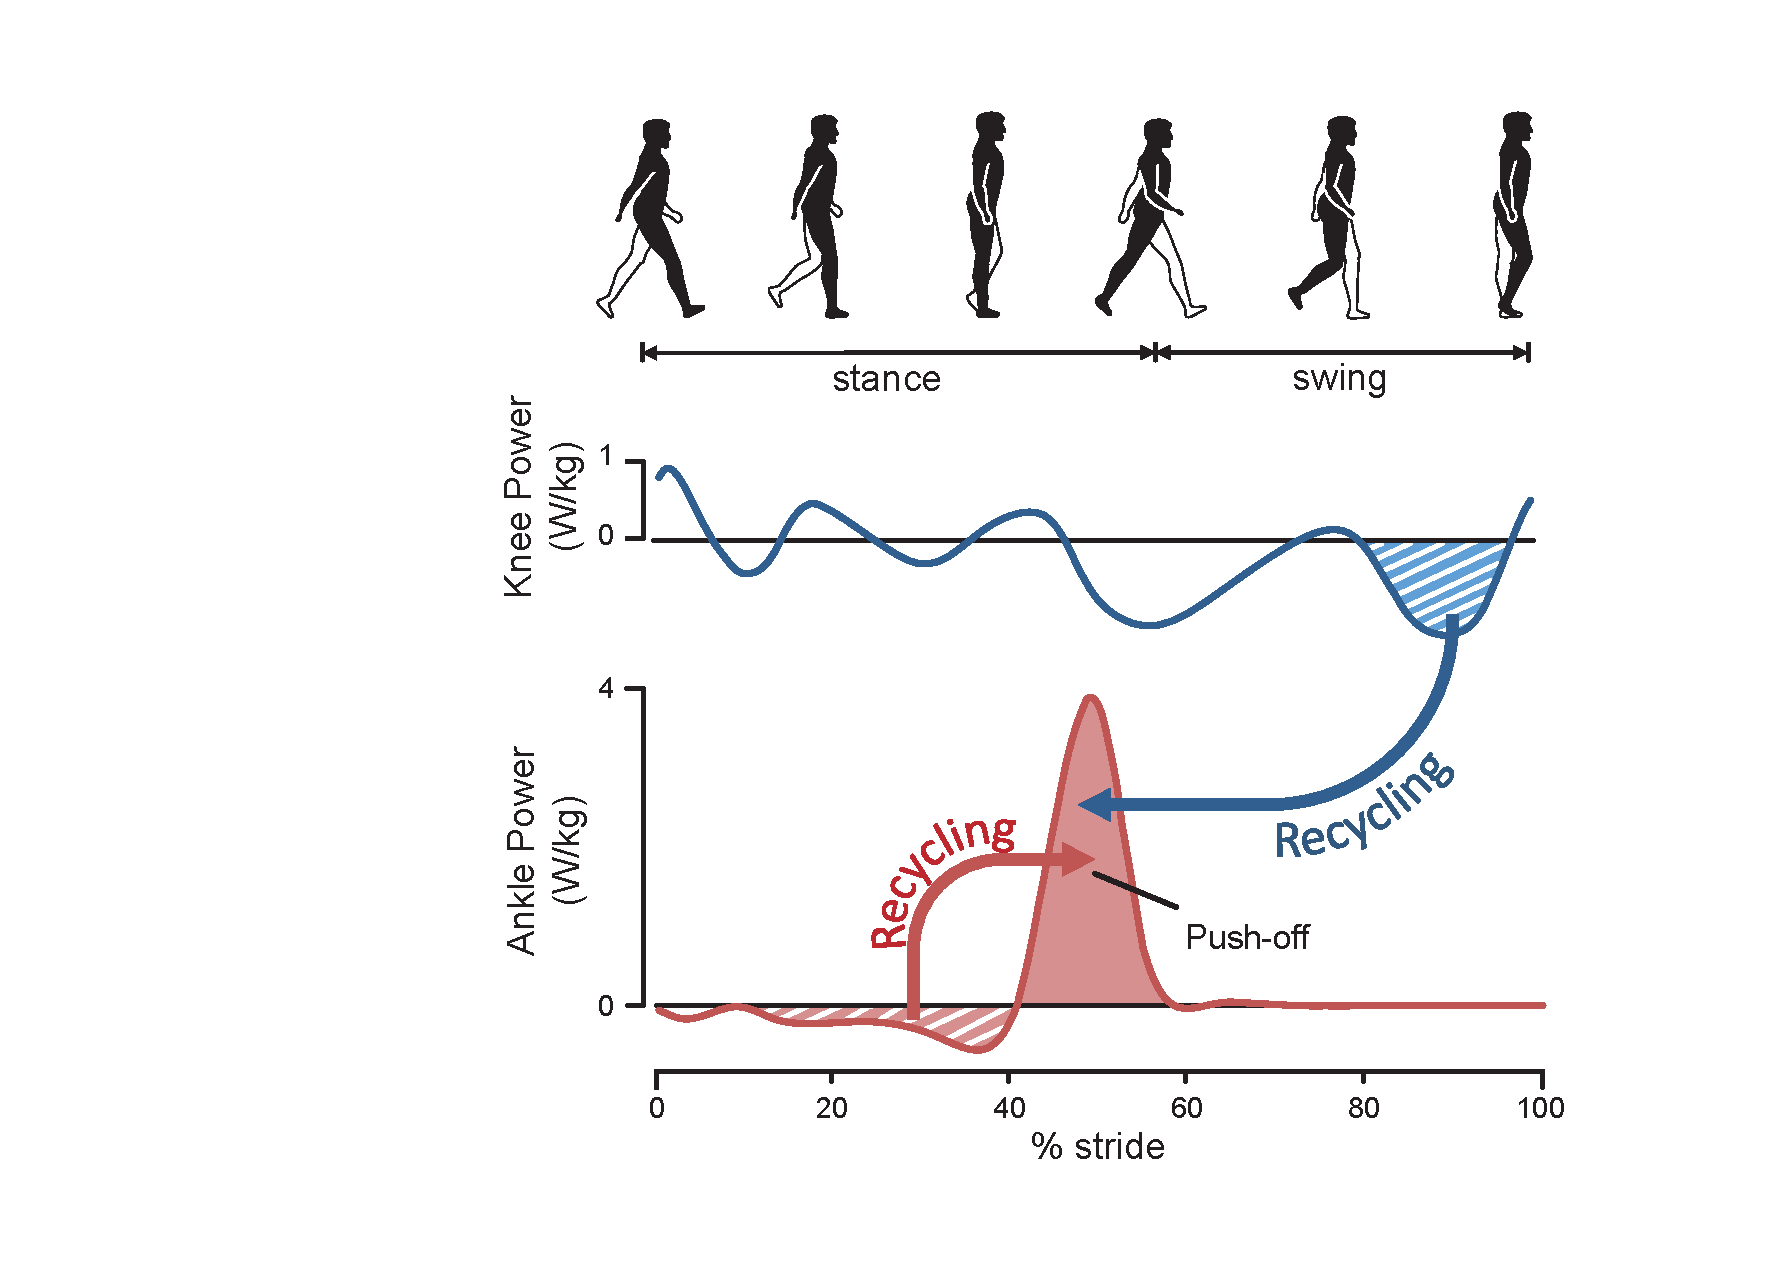
\includegraphics[width=0.45\textwidth]{Figure1.eps}
	\caption{Joint power during human walking.
	Typical work rates of the knee and ankle joints over a gait cycle are shown (adapted from \cite{RN2}).
	The negative work performed by the knee joint in late swing (blue hatched area) and by the ankle joint in mid stance (red hatched area) are possible sources of energy for assisting push-off (red solid area).}
	\label{fig:work}
\end{figure}

Even though this indicates push-off is the best time to supply energy, designing a passive exoskeleton is still challenging since it needs to recycle energy from the human user without adding hindering forces or moments.
Measurements in vivo suggest that a considerable amount of negative work performed by the ankle joint during mid stance dorsiflexion is stored in the Achilles tendon, and used for the following push-off \cite{RN16}.
In this process, the mechanical behavior of the Achilles tendon resembles a spring which is stretched to store energy and then recoils to release energy.
Though no mechanical energy input is needed from muscles, the plantar-flexors (gastrocnemius and soleus) need to provide a counteracting force in order for the angular motion of the ankle to stretch the Achilles tendon for energy storage.
This force is achieved through the muscle isometric contraction, which requires metabolic energy expenditure though no mechanical energy is produced \cite{RN17}.
Thus, in this paper we propose it is beneficial to recycle the negative work from the ankle joint dorsiflexion during stance (red hatched area, 15-40\% Stride, Fig. \ref{fig:work}) with a physical spring and a mechanical fixation of its proximal end, so that plantar-flexors are freed from exerting the counteracting force.

In late swing phase, the knee joint performs a large amount of negative work during extension (blue hatched area, 80-100\% Stride, Fig. \ref{fig:work}).
%In this period, the thigh and shank can be modeled as a jointed double-pendulum pinned at the knee joint\cite{RN2}.
%When knee extends, the lower segment (shank) of the jointed pendulum is returning to its neutral position, being accelerated by gravity.
%To prevent hyper-extension, the knee joint needs to perform negative work to decelerate the shank and this process is accomplished by knee flexors (mainly hamstrings).
This negative work is generated by knee flexors (mainly hamstrings), and is used to decelerate the shank in order to prevent knee joint hyper-extension.
%A device assisting knee in decelerating in principle can bring benefits to human and obtain energy at the same time.
An energy harvester has been designed to use this negative work to generate electricity, which demonstrates very high efficiency with every watt of electricity causing only 0.7 watt of metabolic expenditure increase \cite{RN18}.
This is similar to a regenerative brake decelerating a hybrid car, where the harvested energy can be reused in other applications.
Therefore, we also propose it is beneficial to recycle the negative work performed by the knee joint during late swing extension, and at the same time help knee flexors decelerate the shank.

\subsection{Mechanical Design}

\begin{figure}[b]
	\centering
	\includegraphics[width=8.5cm]{Figure2.eps}
	\caption{Mechanical design of the quasi-passive exoskeleton.
	(a) The schematic of the exoskeleton with key components listed; (b) The exoskeleton worn on a subject.}
	\label{fig:model}   
\end{figure}

There are several design objectives of the exoskeleton.
First, the exoskeleton should properly recycle the negative work from both the knee joint in late swing and the ankle joint in mid-stance, and release the energy to assist ankle plantar flexion during push-off.
Second, because the energy recycled from the knee joint needs to be released approximately half of a gait cycle later (from late swing to the next late stance), the exoskeleton should be able to store the energy for a specific amount of time.
Third, during other periods of a gait cycle when the exoskeleton is not working functionally, it should not hinder the natural movements of the lower limb.
Finally, the exoskeleton should be lightweight and comfortable enough to mitigate the effects of added mass and extra kinematic constraints imposed by the structures.

As shown in Fig. \ref{fig:model}(a), the exoskeleton consists of an ankle brace, a torsion spring with two motor controlled clutches which are integrated into a clutch-spring unit, compression baselayer pants, a pressure insole (not shown) and electronics hardware (not shown).
Fig. \ref{fig:model}(b) shows the quasi-passive exoskeleton worn on a healthy subject.
%The main idea of our device is to use two clutches to control the recycle and release of energy in a torsion spring.
The supporting structure of the exoskeleton is the ankle brace, where the shank and foot parts are connected by a hinged joint.
The torsion spring is used to store recycled mechanical energy, with its two ends fixed to two rotatory clutches which are used to control the timings of recycling and releasing energy.
The clutch-spring unit is fixed to the shank part of the ankle brace.

%When the exoskeleton is working, the two ropes exert resistant moments to the joints during energy recycling, and assistive moments during energy releasing.

\begin{figure}[b]
	\centering
	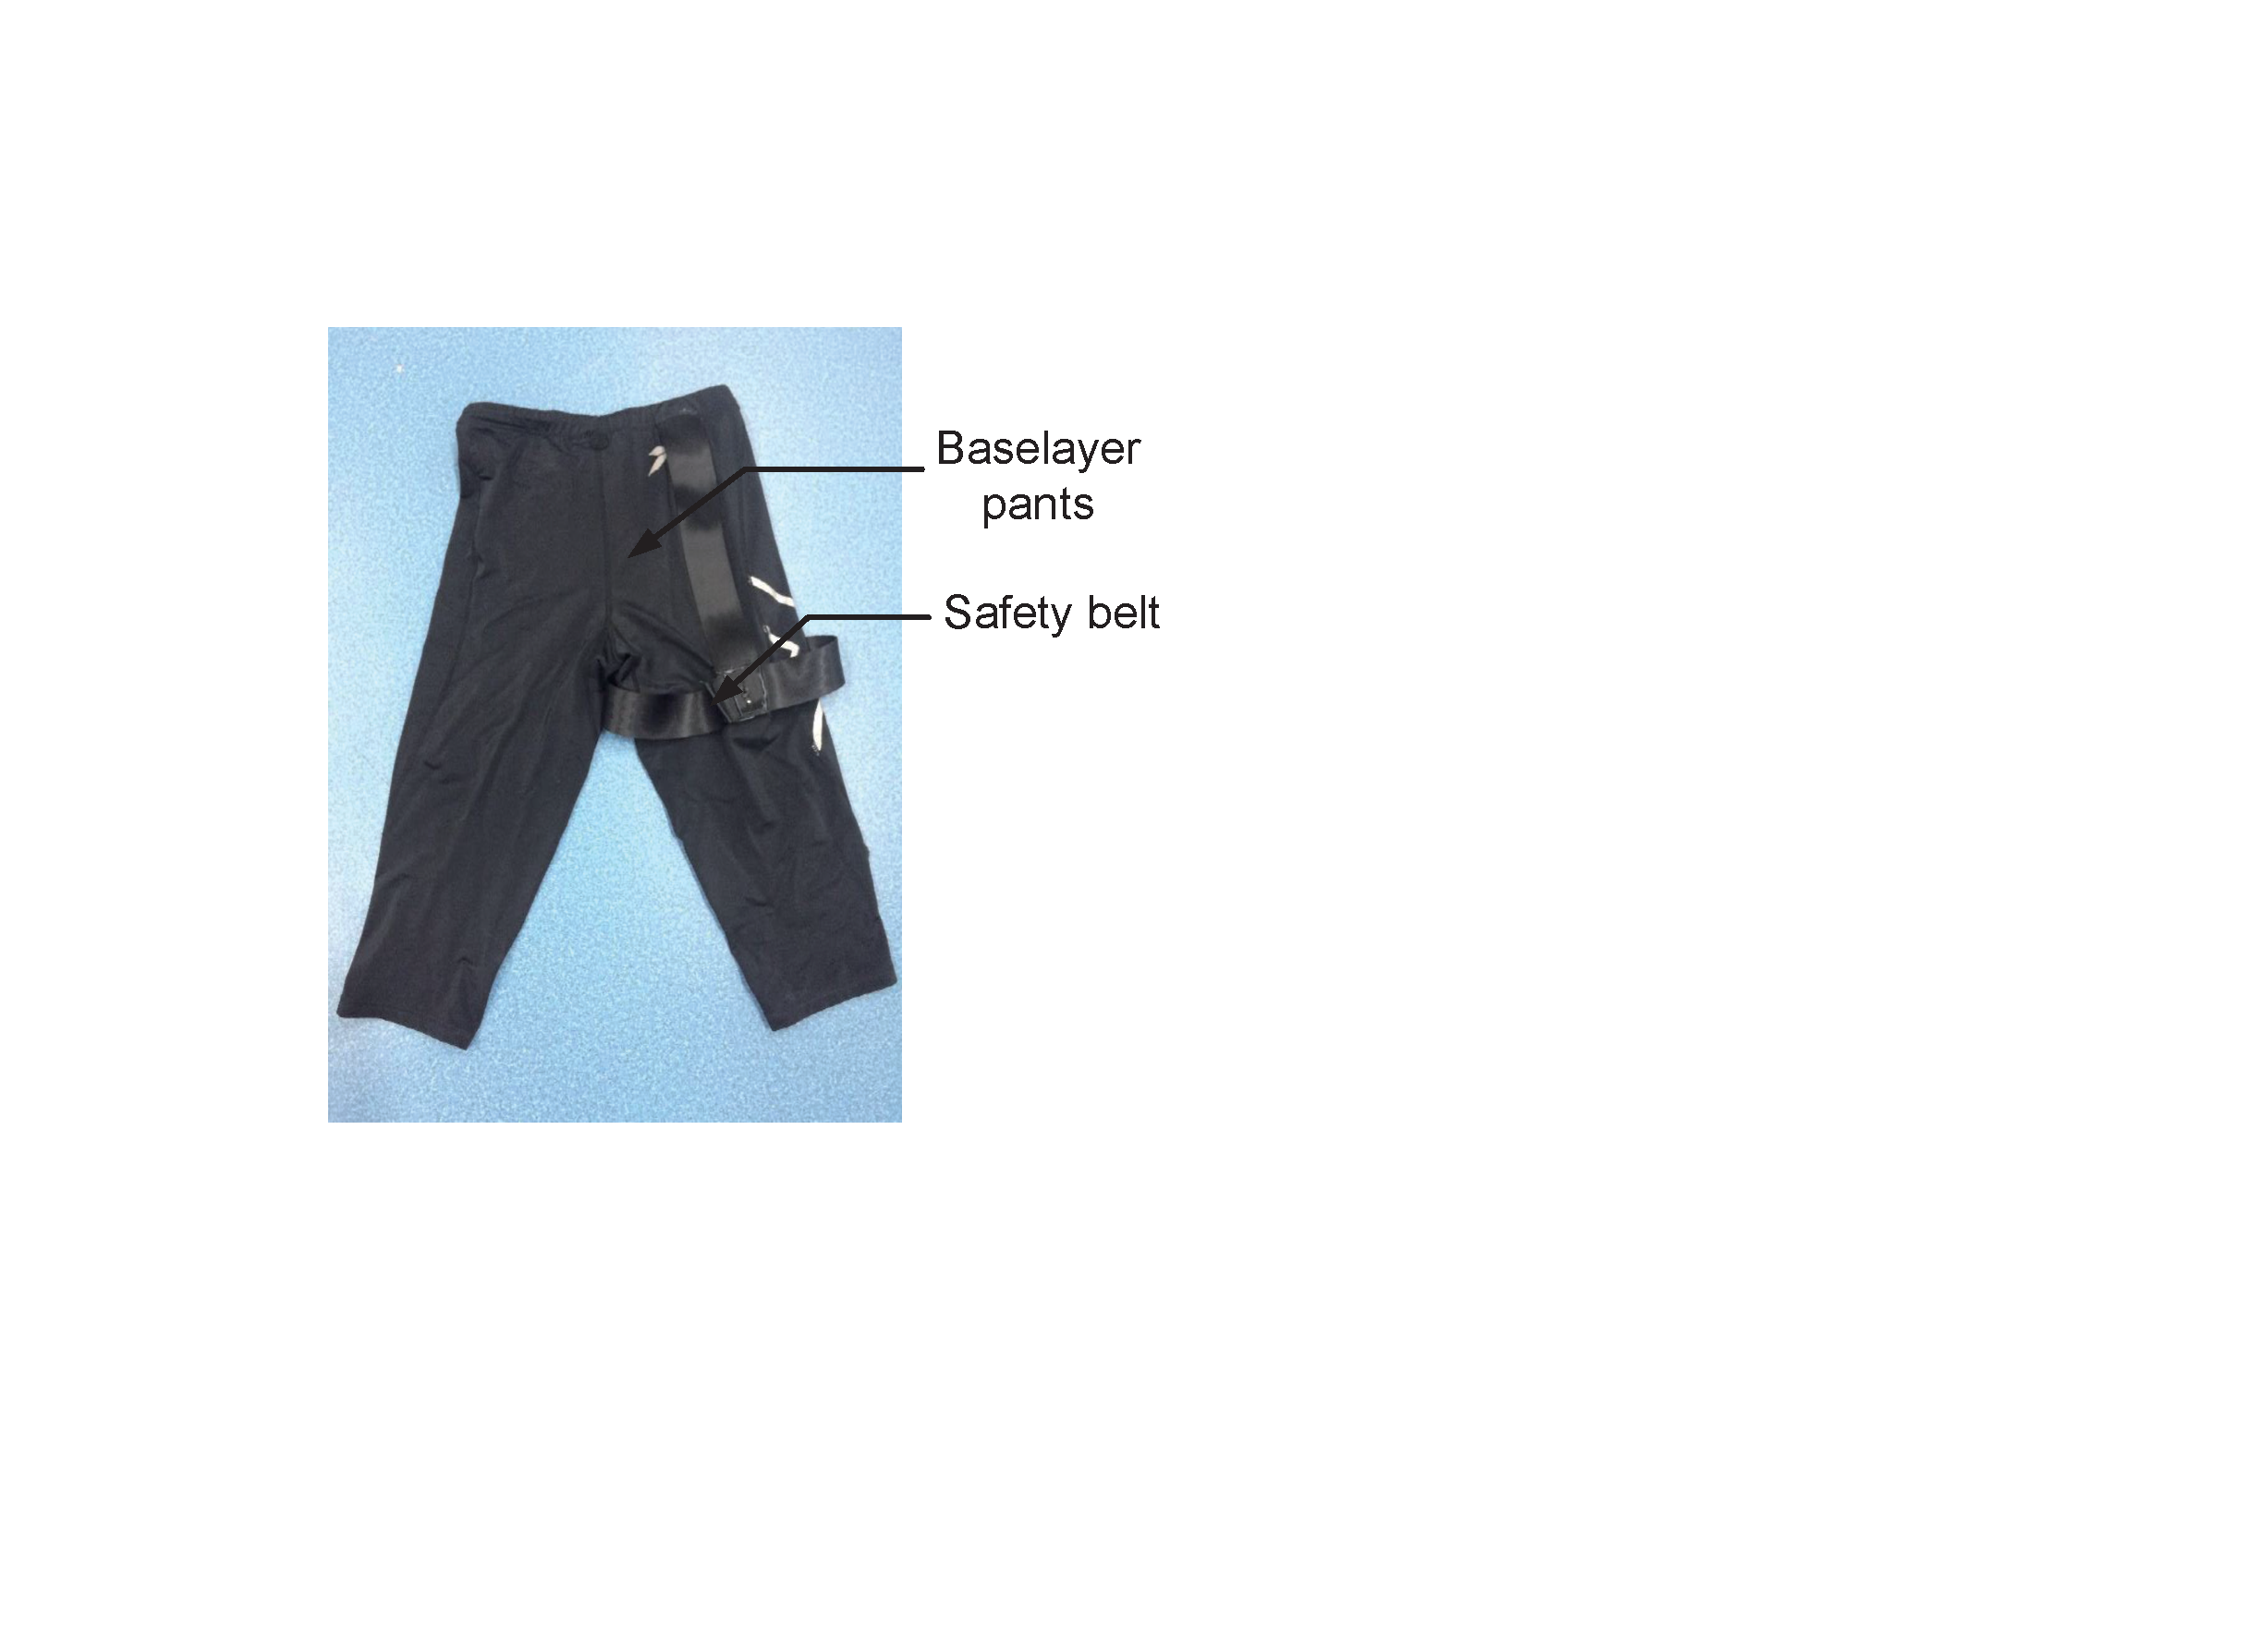
\includegraphics[width=8cm]{Figure3.eps}
	\caption{The thigh fixation: baselayer pants with seat belts sewed into them.}
	\label{fig:pants}   
\end{figure}

Two ropes are connected in series with the torsion spring through the two clutches, and span the knee joint (knee rope) and ankle joint (ankle rope) to exert external moments on these joints.
The lower end of the ankle rope is fixed to the foot part of the ankle brace.
Since the knee joint rotates a larger angle in swing extension than the ankle joint does in late stance plantar flexion, the moment arm at ankle is designed to be large enough to coordinate the traveling distance between the knee and ankle.
Therefore, a bar made of aluminum alloy is extended backwards from the foot part of the ankle brace to provide a large moment arm.

As for the knee rope, it should in principle be rigidly fixed to the thigh.
However, because the thigh tapers distally, the fixation tends to slide off when a downward force is exerted by the rope.
Using a rigid hip brace to tackle this problem is unacceptable to us because of the extra weight it introduces.
Inspired by the soft exo-suit developed in \cite{RN20}, we come up with a slightly compromised solution, which uses baselayer pants to provide an elastic connection to the waist.
In order to minimize the sliding between the pants and the thigh, non-deformable safety belts are sewed into the pants along the paths through which the downward force passes to the waist, as shown in Fig. \ref{fig:pants}.

\begin{figure}[t]
	\centering
	\includegraphics[width=8.5cm]{clutch.eps}
	\caption{Schematics of the clutch-spring unit. (a) The 3D model with key components listed; (b) The exploded view.}
	\label{fig:clutch}   
\end{figure}

The clutch-spring unit is the key component of this exoskeleton, which recycles, stores and releases energy at specific time in a gait cycle.
The 3D model and exploded view of the clutch-spring unit are shown in Fig. \ref{fig:clutch}.
Instead of using an ordinary extension or compression spring, a torsion spring is chosen as the energy storage element, for main considerations that the two clutches and the spring can be encapsulated into a compact unit.
The design of the clutches is based on traditional ratchets, which is inspired by\cite{RN19}.
The position of the pawl is actively controlled through gears by a small servo motor (DS215MG, KST Digital Technology, Guangdong, China) embedded in the shaft of the clutch-spring unit on each side.
The stall torque of the motor is 0.036 Nm.
When the pawl is disengaged, the ratchet wheel can rotate freely in both directions; when the pawl is engaged, the ratchet wheel is only allowed to rotate in the direction stretching the spring.
The motor is rigidly connected to the pawl in the disengaging direction and elastically connected in the engaging direction.
The return elasticity of the pawl is realized by two small ratchet springs assembled between the motor shaft and the gear to push the pawl back, when the ratchet wheel rotates in the allowable direction and potentially disengages the pawl.

Grooves are designed to be outside of the ratchet wheels which serve as pulleys to hold the ropes.
Each end of the torsion spring is fixed to the ratchet wheel by screws and rope clamps.
When the ratchet is locked by engaging the pawl, the direction that releases the spring is prohibited. 
Namely, when both clutches are locked, the elastic energy of the spring is locked into the clutch-spring unit, and no force in the torsion spring passes to the ropes.
The shaft holding the two ratchets serves as the supporting structure of the spring-clutch unit, and is fixed to the shank part of the ankle brace as shown in Fig. \ref{fig:model}(a).
Voids are also designed into the shaft to decrease its weight.

The total weight of the exoskeleton is 832 g, with 623g worn on the shank and 209 g worn on the foot.
A list of the major components with their models/material, weights and locations on the lower limb are shown in Table 1.

%%%%%%%%%%%%%%% begin table   %%%%%%%%%%%%%%%%%%%%%%%%%%

\begin{table}[t]
	\caption{Major components of the exoskeleton}
	\begin{center}
		\label{tab:hardware}
		\begin{tabular}{c c c c}	
			\hline
			\textbf{Component} & \textbf{Model/Material} & \textbf{Mass} & \textbf{Location} \\
			\hline
			Servo motor & DS215MG & 19 g$\times$2 & Shank\\
			Battery & Lithium & 48 g & Foot\\
			Controller & Arduino nano & 21 g & Foot\\
			Clutch-spring & Aluminium alloy & 442 g & Shank\\
			Shank brace & Carbon fibre & 143g & Shank\\
			Foot brace & Carbon fibre & 110 g & Foot\\
			Ankle arm & Aluminium alloy & 30g & Foot\\			
			\hline 
			\textbf{Shank part} & & \textbf{623 g} & \textbf{Shank}\\
			\textbf{Foot part} & & \textbf{209 g} & \textbf{Foot}\\
			\hline
			\textbf{Total} & & \textbf{832 g} & \\
			\hline
		\end{tabular}
	\end{center}
\end{table}

%%%%%%%%%%%%%%%% end table %%%%%%%%%%%%%%%%%%% 

\subsection{Working Cycle of the Exoskeleton}
\label{subsec:Working process}

\begin{figure*}[tb]
	\centering
	\includegraphics[width=17cm]{workingprocess_1.eps}
	\caption{The working process of the exoskeleton in a gait cycle.
	Top: elastic potential energy in the spring; middle: contacting conditions of the heel and toe with the ground, conditions of the knee and ankle clutches; bottom: schematics of working conditions of the quasi-passive exoskeleton.
	The blue arrows indicate the rotating directions of the clutches, and the black arrows indicate the directions of forces in the ropes.}
	\label{fig:workprocess}   
\end{figure*}

The working process of the exoskeleton in a gait cycle is shown in Fig. \ref{fig:workprocess}, where 0\% and 100\% correspond to two successive heel strikes, and 60\% corresponds roughly to toe off.
The description below begins from the swing phase, for the complete energy recycling and releasing cycle of the exoskeleton starts here.
At the beginning of swing phase (Fig. \ref{fig:workprocess}(a)), the two clutches are unlocked.
During late swing (Fig. \ref{fig:workprocess}(b)), the knee joint extends from its maximum flexion angle to full extension.
As a consequence, the knee rope stretches the torsion spring to harvest energy and applies a flexion torque at the knee joint to assist hamstrings in decelerating the shank.
The ankle clutch is locked before the knee joint starts extending in order to decouple the ankle joint, so that the force in the spring is exerted on the clutch instead of the ankle rope.
Before the knee joint fully extends, the knee clutch is locked to store the harvested energy.

In early stance (Fig. \ref{fig:workprocess}(c)), the ankle joint naturally achieves foot flat through slight plantar flexion motions, and the knee joint also undergoes slight flexion motions, both of which are in the direction that releases the energy in the torsion spring.
However, because the two clutches remain locked in this period, both joints are decoupled from the torsion spring.
Therefore, the recycled energy in the torsion spring is preserved and no force is passed to the ropes causing hindering moments on the knee and ankle joints.

When the shank approaches its vertical position in mid stance (Fig. \ref{fig:workprocess}(d)), the torsion spring begins to be stretched again by the ankle rope to recycle energy from ankle.
The start of recycling is determined by the original ankle rope length, which can be adjusted to change the amount of energy recycled from ankle.
It is important to unlock the ankle clutch during mid stance when the ankle rope is stretching the torsion spring, because the pawl is unloaded and only a small torque from the motor is needed to disengage it.
The knee clutch keeps locked throughout this period.

In late stance (Fig. \ref{fig:workprocess}(e)), a burst of positive power is needed at the ankle joint to redirect the velocity of the COM of body.
In this process, the force in the torsion spring is passed to the ankle rope and exerts a plantar flexion torque at the ankle joint to perform positive mechanical work.
As ankle plantar flexion progresses, the torsion spring recoils and the previously recycled energy is finally released.
The ankle clutch keeps unlocked throughout this process to allow force transmission between the torsion spring and the ankle joint, while the knee clutch keeps locked to decouple the knee joint from the spring.

After push-off, both ratchet wheels have rotated in the same direction for some angles from their initial positions.
This means they should return to their initial positions to prepare for the next working cycle during initial swing (Fig. \ref{fig:workprocess}(a)).
In this period, because both pawls are disengaged, we can simplify the spring-clutch unit as a rigid body.
That is, if one ratchet wheel returns to its initial position, the other returns automatically.

We use a return spring to accelerate the returning process of the two ratchet wheels, which is connected between the ratchet wheel on the knee side and the shaft of the spring-clutch unit.
The return spring drags the two ratchet wheels back to their initial positions.
An almost negligible side-effect is that when the torsion spring is stretched in late swing, the return spring is also stretched, which causes some energy wasted.
However, the return spring can be much softer than the torsion spring provided it can overcome the friction force between the ratchet wheels and the shaft.
Therefore, the amount of energy wasted by the return spring should be small. 


\subsection{Control System Design}


\begin{table*}[b]
	\centering
	\newcommand{\tabincell}[2]{\begin{tabular}{@{}#1@{}}#2\end{tabular}}
	\renewcommand{\arraystretch}{1.3}
	\caption{Allowable time interval and plantar pressure criteria of clutch motions}
	\begin{center}
		\label{tab:control}
		\begin{tabular}{c c c c} 
			\hline
			\hline
			\multirow{2}{*}{\textbf{Clutch motion}} &  \multicolumn{2}{ c }{\textbf{Allowable time interval} (\% gait cycle)} & \multirow{2}{*}{\shortstack{\textbf{Plantar pressure criteria} \\ 
			(55 strides per minute)}} \\ \cline{2-3}&\textbf{Start from} & \textbf{End before}\\
			\hline
			Ankle clutch locks & \tabincell{c}{End of push-off \\ (60\%)} & \tabincell{c}{Beginning of knee extension \\ (75\%)} & \tabincell{c}{0.1s after plantar \\ pressure disappears}\\
			Knee clutch locks & \tabincell{c}{Beginning of knee extension \\ (75\%)} & \tabincell{c}{Heel strike \\ (100\%)} &\tabincell{c}{0.2s after plantar\\ pressure disappears}\\
			Ankle clutch unlocks & \tabincell{c}{Ankle in its neutral position \\ (around 25\%)} & \tabincell{c}{Beginning of push-off \\ (40 \%)} &\tabincell{c}{0.1s after forefoot\\ pressure appears}\\
			Knee clutch unlocks & \tabincell{c}{End of push-off \\ (60\%)} & \tabincell{c}{End of push-off \\ (60\%)} &\tabincell{c}{Right after plantar \\ pressure disappears} \\
			\hline
			\hline
		\end{tabular}
	\end{center}
\end{table*}


The control system of the exoskeleton (shown in Fig. \ref{fig:control}) includes a micro controller (Arduino NANO), two motors, a pressure insole, and an 800 mA$\cdot$h lithium battery.
The input voltage of the Arduino NANO and the servo motors are 6V-8V and 4.5V-8.5V respectively.
So a 8V lithium battery is used to power the control system.
The 5V output from the micro controller is used as the input voltage of the plantar pressure sensors. 

Different from active exoskeletons, the control scheme of the quasi-passive exoskeleton is not to apply torques at lower limb joints by actuators, but to specify the timings to lock and unlock the two clutches.
It is reasonable to use the plantar pressure information for this control objective, as the most frequently referenced gait event is push-off.
The pressure insole is placed between the ankle brace and foot to detect heel strike, toe off and mid-stance events.
Six force sensing resistors are sewed into the insole, with four of them placed under the forefoot to detect toe off, and the rest two placed under the heel to detect heel strike.
Because precise measurements are not needed, the four sensors under forefoot and the two under heel are electronically wired in parallel respectively. 

\begin{figure}[t]
	\centering
	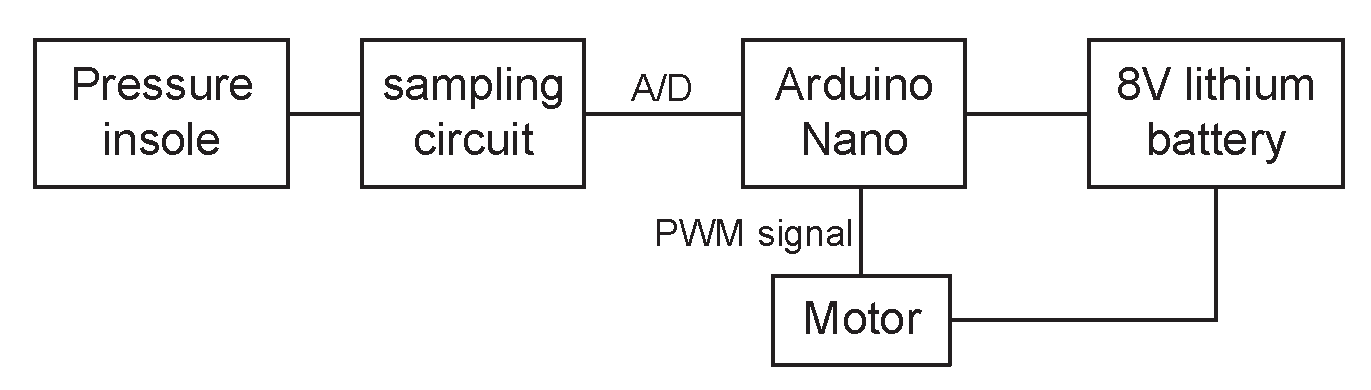
\includegraphics[width=8.5cm]{control.eps}
	\caption{The control system of the exoskeleton.}
	\label{fig:control}   
\end{figure}

Based on the discussions in Section \ref{subsec:Working process}, locking and unlocking the ankle clutch as well as locking the knee clutch can be performed within some time intervals, whereas unlocking the knee clutch should be performed at a specific moment in a gait cycle.
The detailed descriptions of the allowed time intervals to perform these clutch movements, and how these timings are deduced from the plantar pressure are listed in Table \ref{tab:control}.

In this current study, the timings of clutches are designed according to the normal step frequency at 55 strides (full gait cycles) per minute (corresponding to around 1.3 m/s walking speed).
More specifically, the ankle and knee clutches should lock between 60\% to 75\%, and 75\% to 100\% of a gait cycle (roughly 0s-0.2s and 0.2s-0.4s after toe off), which motivates the choices of the time delays listed in Table \ref{tab:control} after considering the delay in the mechanical system.
Similarly, the timings for unlocking the ankle and knee clutches are chosen based on the detected mid-stance and toe off from the plantar pressure.
The choices of time delays are justified by wearers being able to walk with the exoskeleton in a natural manner.

\subsection{Parameter Design}

\label{sec:parameter design}

Human walking is highly optimized by evolution, thus improper moments applied at the joint may result in undesirable consequences.
It has been found that even though the activities of plantar flexors assisted by an exoskeleton do not disappear completely, the activities of dorsiflexors begin to increase to counteract the effect of the exoskeleton, which leads to increased metabolic expenditure \cite{RN4}.
Such muscle behavior is referred to as muscle co-contraction, which also happens between hamstrings and quadriceps, a pair of antagonistic muscle groups on the thigh.
Hence, the best assisting strategy lies on the boundary at which the co-contraction is just about to happen \cite{RN22}. 

The maximum amount of negative power and work that the exoskeleton recycles from the knee and ankle joints are determined by referring to existing devices.
From the experiment data of human subjects in \cite{RN5,RN18}, they are roughly estimated as follows:
%While reducing the energy recycled in the ankle joint dorsiflexion to avoid muscle antagonism, the peak assisting power of the quasi-passive exoskeleton at late stance should be as large as possible. Referring to the knee energy harvester device designed by Donelan \emph{et al.}, the exoskeleton should be avoid to apply excessive moment to the knee joint at late swing phase. We set the boundary conditions for the exoskeleton as following (assuming the wearer weighs 65 kg):

(1) The peak negative power applied by the exoskeleton to the knee joint should be less than 0.3 W/kg during knee extension in late stance, and the negative work recycled from the knee joint should not exceed 35\% of the biological negative work;

(2) The peak negative power applied by the exoskeleton to the ankle joint should be less than 0.2 W/kg during dorsiflexion in mid stance, and the negative work recycled from the ankle joint should not exceed 10\% of the biological negative work.

\begin{figure}[t]
	\centering
	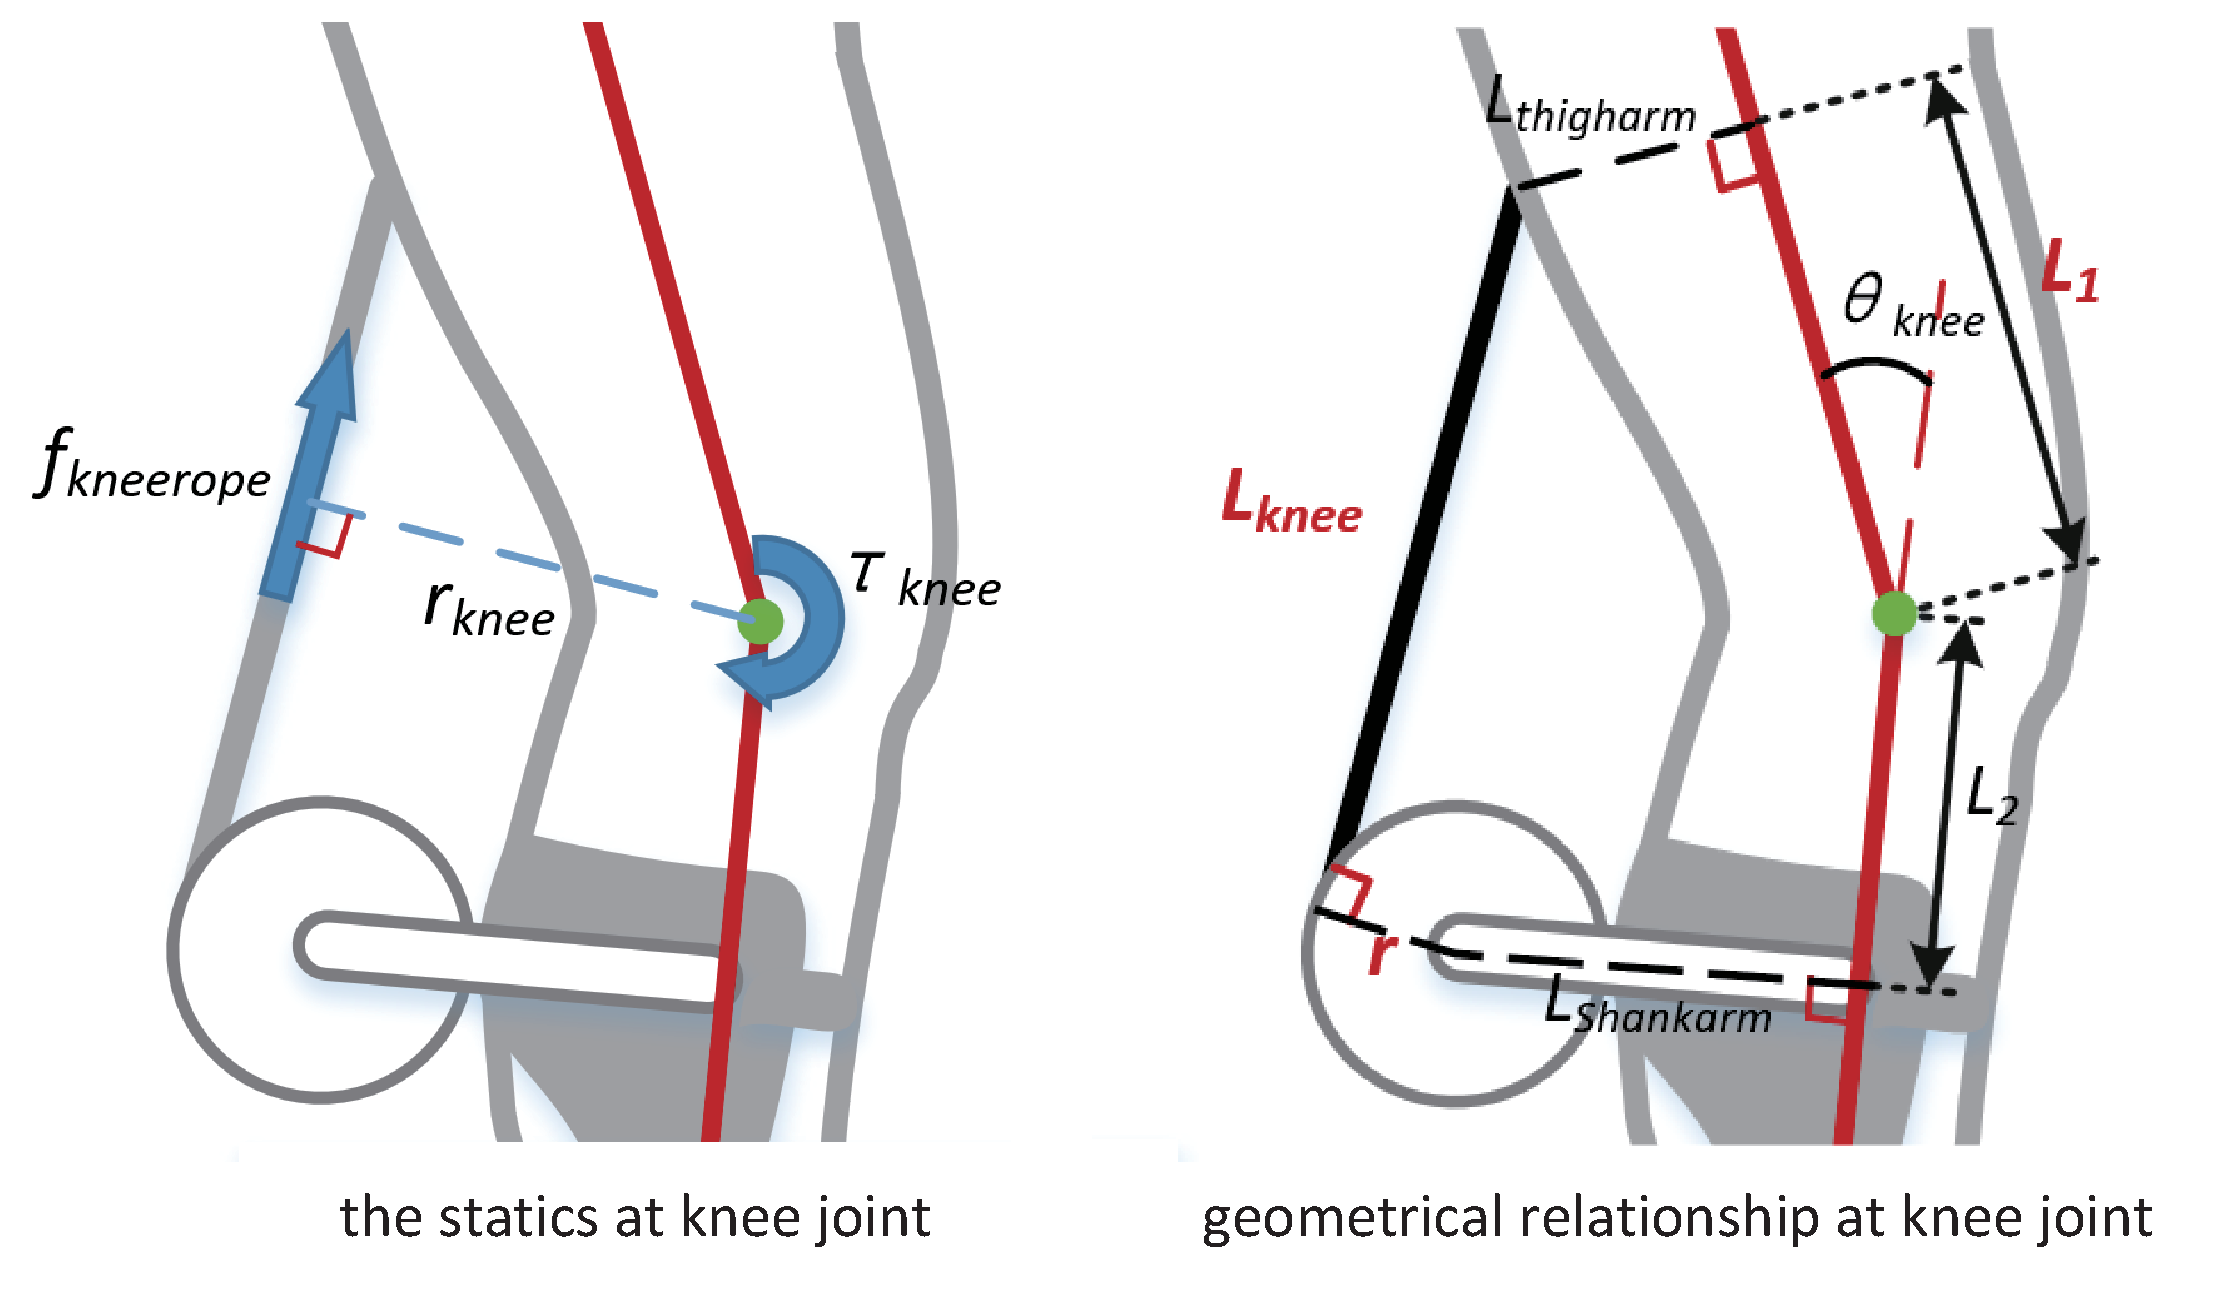
\includegraphics[width=8.5cm]{kneeparameters.eps}
	\caption{The statics and geometric relationships between the exoskeleton and knee joint.}
	\label{fig:kneeparameters}
\end{figure}

\begin{figure}[t]
	\centering
	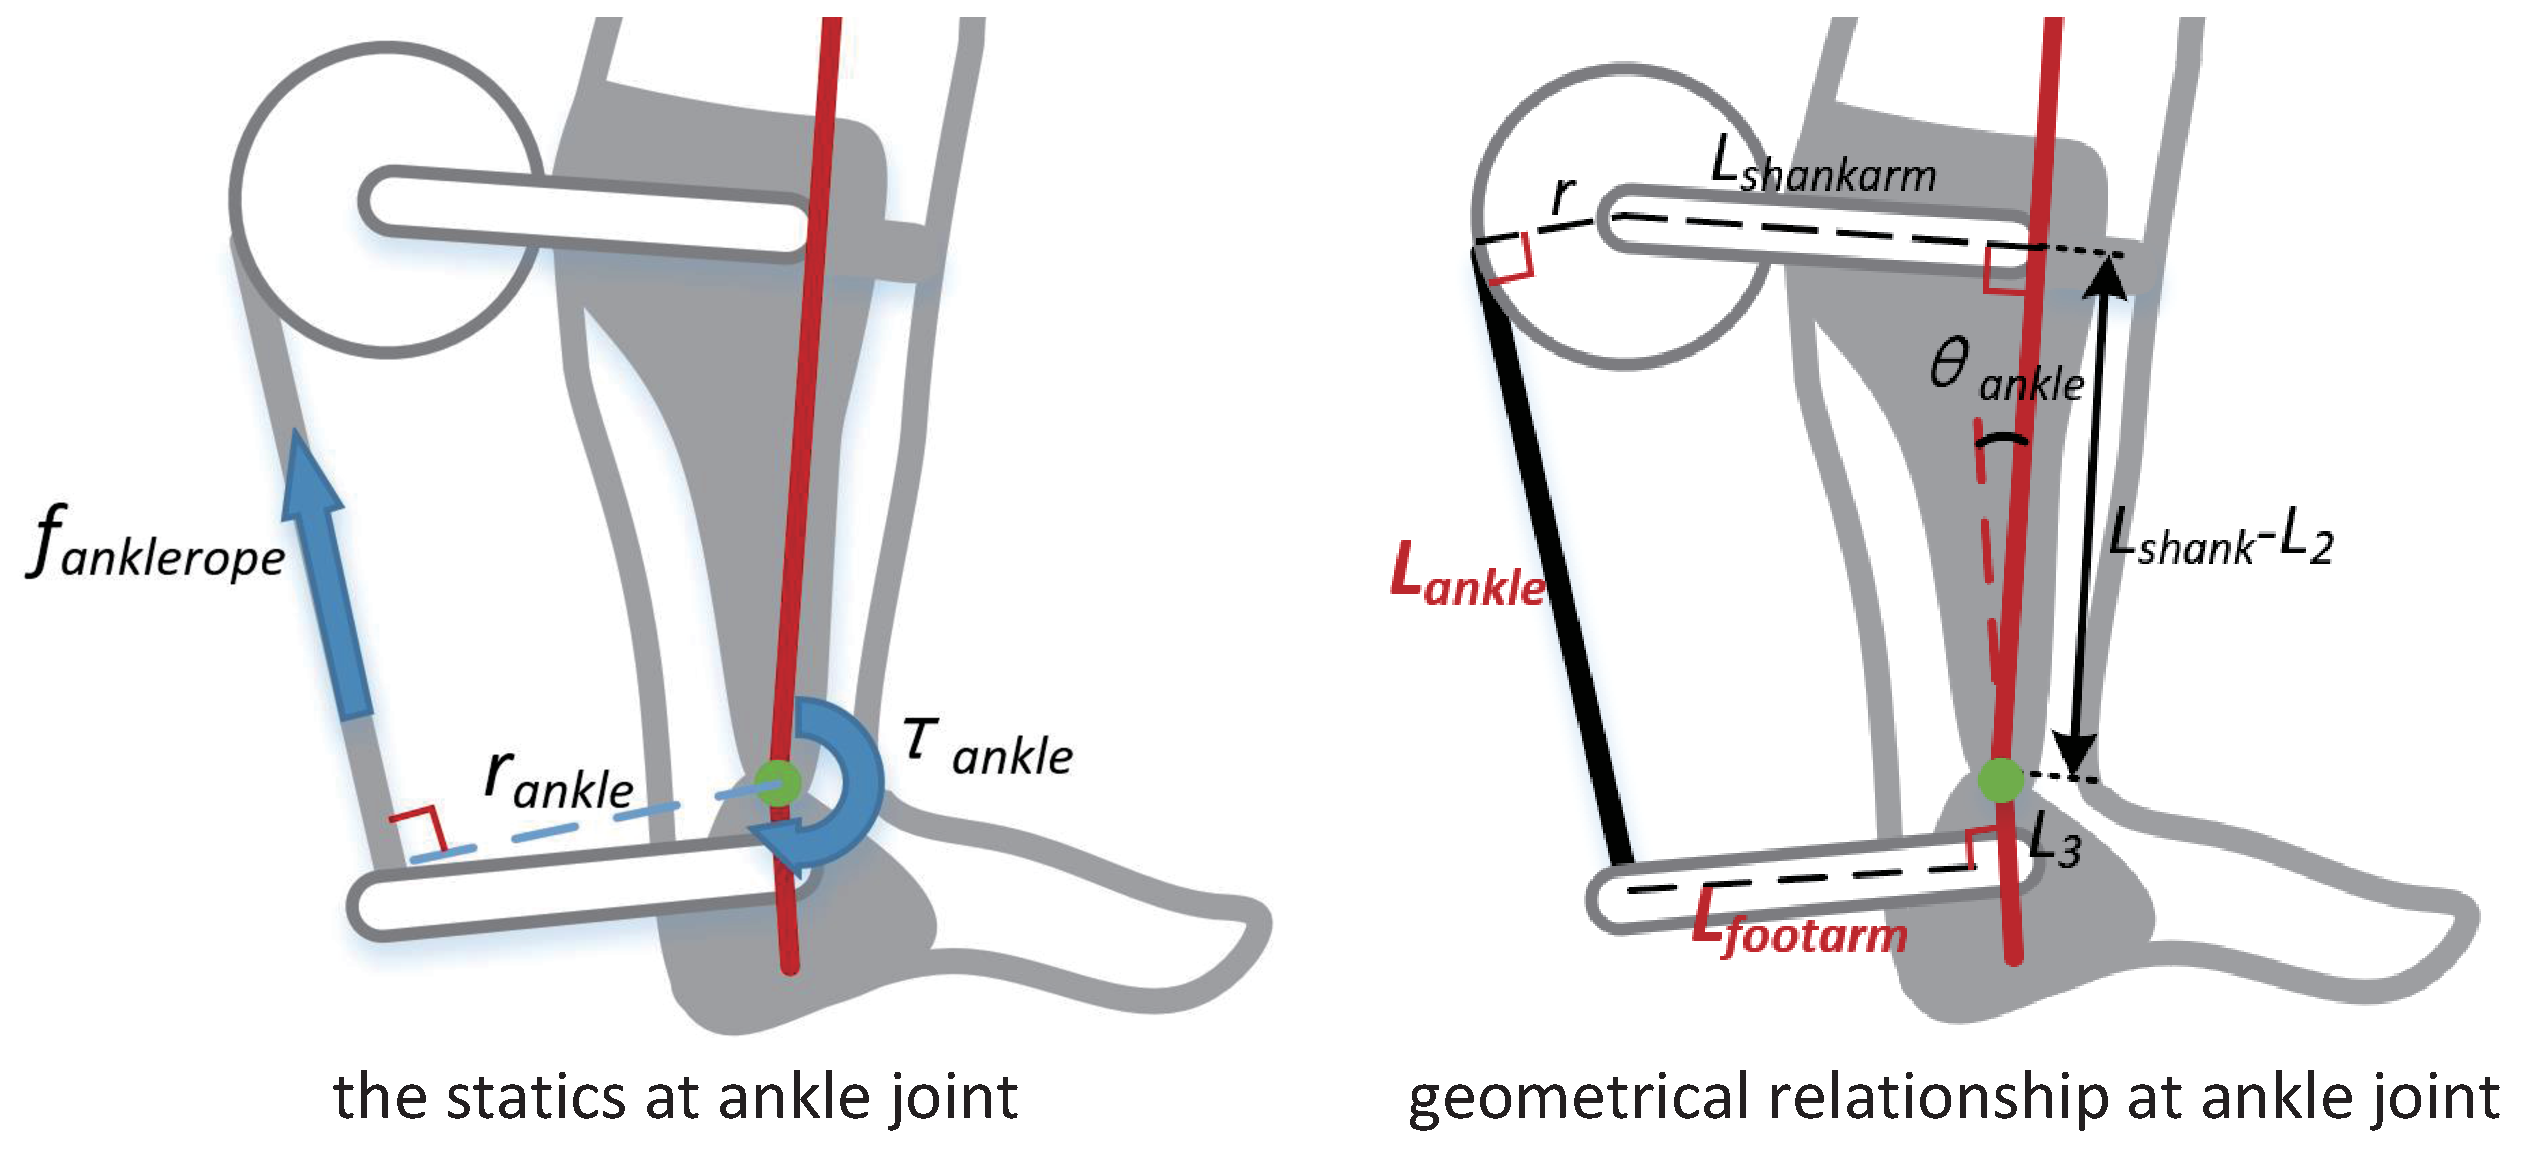
\includegraphics[width=8.5cm]{ankleparameters.eps}
	\caption{The statics and geometric relationships between the exoskeleton and ankle joint.}
	\label{fig:ankleparameters}
\end{figure}

%The ratchet radius is $r$. The distance from the fixed point of the thigh to the center of the knee is $L_\textrm1$. The distance between the fixed point of the ankle brace to the center of the knee is $L_\textrm2$. The initial knee rope length is $L_\textrm{kneerope}^0$. The vertical distance from the center of the clutch-spring unit to the fixed point of the ankle brace is $L_\textrm{shankarm}$ (fixed to 10 cm). The distance between the thigh fixed point and the knee ratchet connection point can be calculated as $L_\textrm{knee}$ by the geometrical relationship. The length of the foot support bar is $L_\textrm{footarm}$.  The initial ankle rope length is $L_\textrm{anklerope}^0$. The distance between the foot fixed point and the ankle ratchet connection point can be calculated as $L_\textrm{ankle}$.

The statics and geometric relationships between the exoskeleton and joints are shown in Fig. \ref{fig:kneeparameters} and \ref{fig:ankleparameters}.
The forces in the two ropes spanning the knee and ankle joints while they are performing negative work are calculated as follows:
\begin{gather}
	f_\mathrm{kneerope} = \frac{k(L_\mathrm{kneerope}-L_\mathrm{kneerope}^0)}{r^2} \\
	f_\mathrm{anklerope} = \frac{k(L_\mathrm{anklerope}-L_\mathrm{anklerope}^0+\Delta L_\mathrm{kneerope})}{r^2},
\end{gather}
where $r$ is the radius of torsion spring, $k$ is its stiffness coefficient, $L_\mathrm{kneerope}$, $L_\mathrm{anklerope}$ and $L_\mathrm{kneerope}^0$, $L_\mathrm{anklerope}^0$ are the lengths and initial lengths of the two ropes, and $\Delta L_\mathrm{kneerope}$ is the final length change of the knee rope after knee extension in late swing phase.

Then, using the notations in Fig. \ref{fig:kneeparameters} and \ref{fig:ankleparameters}, the negative power and work of the exoskeleton applied to the knee and ankle joints are
\begin{gather}
	P_\mathrm{knee} = r_\mathrm{knee}f_\mathrm{kneerope}\dot{\theta}_\mathrm{knee} \\
	P_\mathrm{ankle} = r_\mathrm{ankle}f_\mathrm{anklerope}\dot{\theta}_\mathrm{ankle} \\
	W_\mathrm{knee} = \frac{1}{2}k\Delta L_\mathrm{kneerope}^2 \\
	W_\mathrm{ankle} = \frac{1}{2}k(\Delta L_\mathrm{kneerope}+\Delta L_\mathrm{anklerope})^2 - W_\mathrm{knee}
\end{gather}
where $\dot{\theta}_\mathrm{knee}$, $\dot{\theta}_\mathrm{ankle}$ are the joint velocities, and $\Delta L_\mathrm{anklerope}$ is the final length change of the ankle rope after dorsiflexion in mid stance.
From the normal values of joint velocities and angles during walking at around 1.3 m/s, and the geometric relationships, we calculate the peak negative power and work of the exoskeleton as functions of the design parameters listed in Table \ref{tab:Exoskeleton parameters}.
Then based on the pre-determined upper bounds on the negative power and work, and assuming the wearer weighs around 65 kg, we choose the design parameters accordingly.

%The energy that the exoskeleton recycled is:
%\begin{equation}
%W_\textrm{in}=W_\textrm{out}=\frac{1}{2}k(\phi(t_4))^2
%\end{equation}

%The torque and power are proportional to the stiffness coefficient of the spring. In the process of parameter selection, we first fix the stiffness coefficient of 1 Nm/rad. Then determine the shape of the assist power curve by adjusting the hardware parameters. The final selected parameter are shown in table \ref{tab:Exoskeleton parameters}.

\begin{table}[t]
	\caption{Exoskeleton parameters}
	\begin{center}
		\label{tab:Exoskeleton parameters}
		\begin{tabular}{c c}	
			\hline
			\textbf{Description } & \textbf{Value} \\
			\hline
			Spring stiffness & 1 Nm/rad\\
			$r$ & 37.5mm\\
			$L_\textrm1$ & 110mm\\
			$L_\textrm2$ & 200mm\\
			$L_\textrm{anklerope}^0$ & 250mm\\
			$L_\textrm{shankarm}$  & 100mm\\
			$L_\textrm{anklerope}^0$ & 280mm\\
			$L_\textrm{footarm}$ & 200mm\\
			\hline
		\end{tabular}
	\end{center}
\end{table}

%%%%%%%%%%%%%%%% end table %%%%%%%%%%%%%%%%%%% 

The stiffness of the torsion spring can be used to change the maximum work that is able to be recycled by the exoskeleton without exaggerating the geometric parameters.
In this current prototype, the stiffness is chosen as 1 Nm/rad, which results in some appropriate geometric lengths, and the final design of the exoskeleton is of compact dimensions as shown in Fig. \ref{fig:model}.
For wearers weighing more than 65 kg, a larger torsion spring stiffness may be chosen because more energy is needed to be stored in the exoskeleton, and vice versa.

\section{Experimental Evaluation}
\label{sec:experiment}  

\subsection{Experimental Protocols}

Eight male subjects (average age = $21.25 \pm2.49$ years) who were free from musculoskeletal injuries or diseases participated in the study.
The average body weight and height of the subjects were $66.88\pm3.91$kg and $1.77\pm0.03$ m.
Subjects gave informed consents that were approved by the local Medical Ethical Committee before participation.
The subjects were permitted to suspend the experiment at any time. 

Three walking conditions were conducted in the present study: (i) normal walking without exoskeletons (NO\_EXO), (ii) walking with the operating exoskeleton (EXO\_ON), and (iii) walking with the exoskeleton but without the knee or ankle ropes (EXO\_OFF).
The NO\_EXO condition was used as the baseline, and the EXO\_OFF condition was included to evaluate the exoskeleton without being affected by its own weight and the kinematic constraints imposed by the foot, shank braces, and the artificial ankle joint.
The participants wore the exoskeleton only on the right leg for both the EXO\_ON and EXO\_OFF conditions.
During the experiment, all participants wore the same running shoes on both feet. 

In order to make the participants sufficiently adapted to the exoskeleton, each participant completed a training session one day before the formal data collection.
During the training, each participant completed two practice walking sessions each for 20 minutes under the EXO\_ON and EXO\_OFF conditions.
The training time was determined to be similar to \cite{RN5}.
On the same day before the data collection, the participants were asked to walk under the EXO\_ON and the EXO\_OFF conditions for another one or two minutes for warming up.

During the data collection, ten successive trials were conducted under each walking condition for one subject.
Each trial was to walk along a 12 meter long walkway.
In order to avoid any ordering effects, the three conditions were tested in random orders.
The participants were asked to rest for five minutes between two walking conditions.
In both training and data collection sessions, a metronome was used to control the step frequency to be around 110 steps (half gait cycle) per minute.
The average walking speed of the participants during data collections was 1.3$\pm$0.1 m/s.

\subsection{Data Collection and Processing}

\begin{figure}[bt]
	\centering
	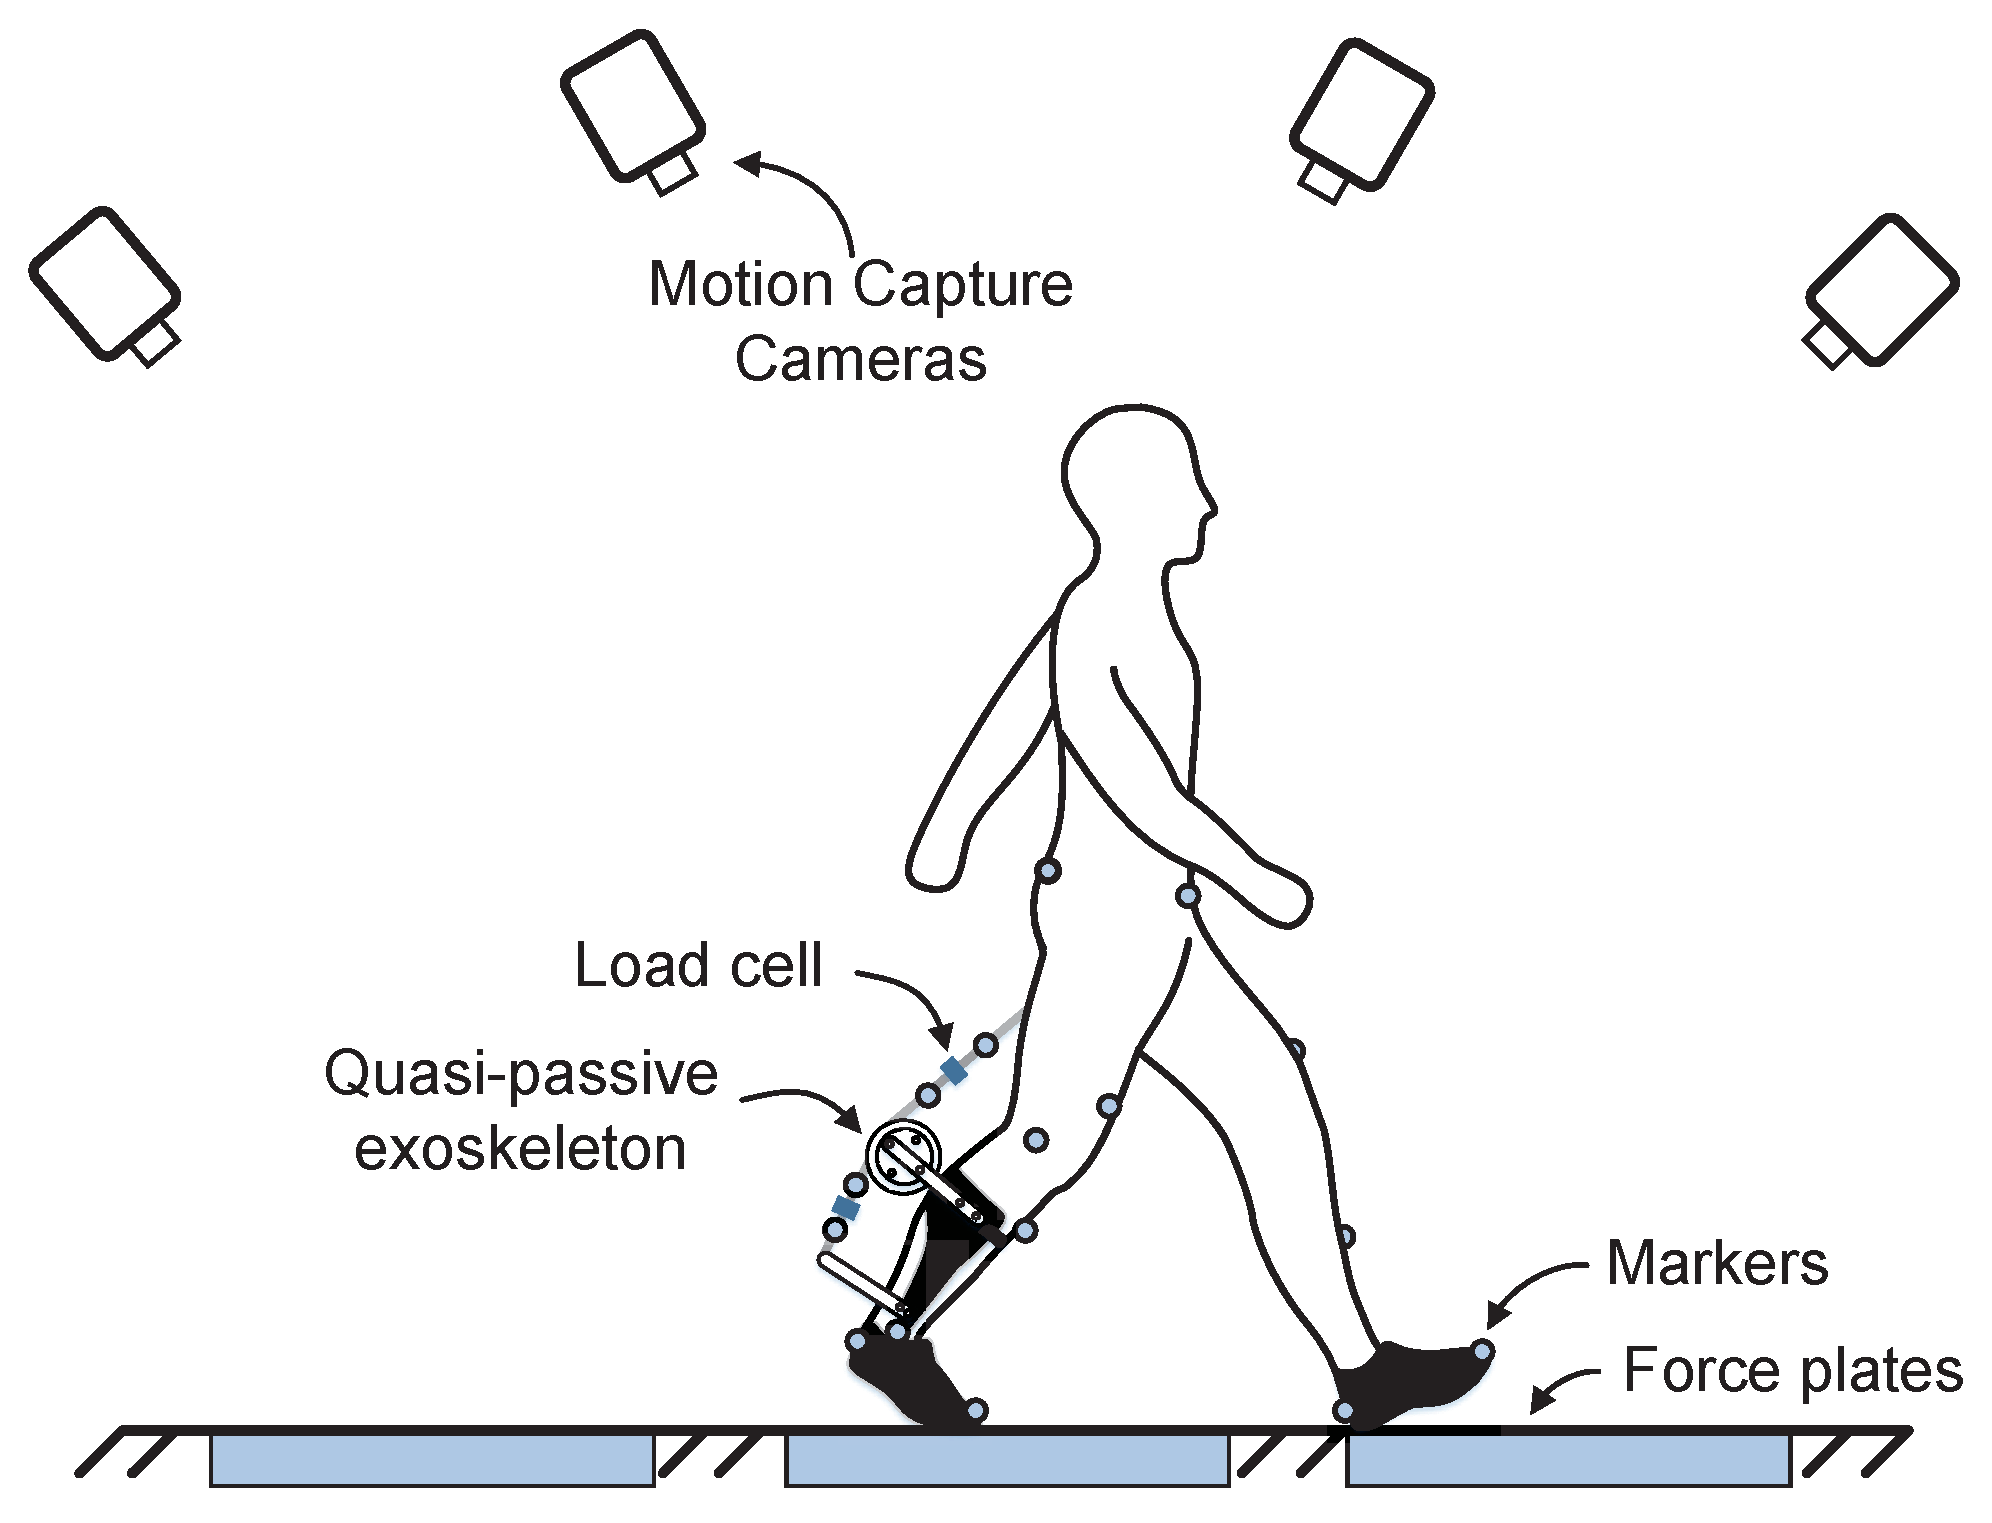
\includegraphics[width=8.5cm]{environment.eps}
	\caption{Experiment setup.
	A motion capture system (including six cameras, fifteen makers on the subject and two markers on each rope) was used to collect walking kinematics data, and three force plates were used to measure ground reaction forces.
	Two load cells were used to measure the forces in the two ropes.
	Subjects wore the exoskeleton only on the right leg.
	Markers were placed on lower limbs following the Helen Hayes marker set.}
	\label{fig:Environment}
\end{figure}

The experiment setup is shown in Fig. \ref{fig:Environment}.
The kinematic data of lower limbs were recorded by 15 reflective markers attached on the participates following the Helen-Hayes marker set \cite{RN24} without the upper body.
The markers were tracked by a 3D motion capture system with six cameras (Motion Analysis, Santa Rosa, CA, USA) at 120 Hz, and analyzed by the Cortex Motion Analysis Software.
Simultaneously, ground reaction forces (GRFs) were sampled at 1200 Hz by three multi-axis force plates (400$\times$600 mm$^{2}$, Bertec, Columbus, OH, USA), which were embedded in a 12 meter long and 1 meter wide straight walkway.
Trials were recognized as successful only if the subject contacted a force plate with the complete right foot.
In the EXO\_ON condition, two load cells (LCM300 Series, Futek, Irvine, CA, USA) were used to measure the forces in the two ropes.
Matched analog amplifiers (Futek, Irvine, CA, USA) and a data acquisition module were used to magnify and collect the analog force signals at 200 Hz.
Additionally, two markers were attached to each rope to measure the moment arms at the knee and ankle joints.

In post processing, the marker positions and the GRFs were filtered by a zero-lag third order Butterworth low-pass filter with the cutoff frequency at 6 Hz and 30 Hz respectively.
We obtained joint angles, velocities and accelerations from the marker positions with inverse kinematics calculations in Matlab (MathWorks, Natick, MA, USA) using the algorithm in \cite{RN24}.
The anthropometric data for each subject were measured, and the lower limb segment mass and COM were adapted from the normal relative body segment mass data measured with college aged males in \cite{de1996adjustments}.
Total joint moments and power were calculated from the kinematic data and GRFs using the Newton-Euler method \cite{kane1985dynamics}.

For the EXO\_ON condition, the total joint moments and power consisted of two parts: the exoskeleton part produced by the torsion spring, and the biological part produced by muscles.
The total joint moments were those obtained from the inverse dynamics analysis, and the total joint power was calculated by the dot product of the joint velocity and moment.
The exoskeleton moments were calculated by the product of the forces recorded by the load cells and the corresponding moment arms measured from the two markers on the ropes.
The moment arms were defined as the distance between the ropes and the joint centers, i.e. $r_\mathrm{knee}$ and $r_\mathrm{ankle}$ in Fig. \ref{fig:kneeparameters} and Fig. \ref{fig:ankleparameters}.
Then the exoskeleton power was calculated by the product of joint velocities and the exoskeleton moments.
Biological joint moments and power during the EXO\_ON condition were defined by subtracting the exoskeleton parts from the total joint moments and power.
For the NO\_EXO and the EXO\_OFF conditions, the biological joint moments and power were the same as the total joint moments and power.
The work during a specific period was obtained by integrating the corresponding power over time.

Joint kinematics and kinetics results were segmented into individual strides based on heel-strike events detected from GRFs.
All moments and power were normalized by the weights of the subjects.
For each subject in each condition, the results were averaged across successful trials from heel strike (0\%) to the next heel strike (100\%).
Then the results were further averaged across the eight subjects.
In order to compare the angles, moments and power of the lower limb joints among the three walking conditions (EXO\_ON, EXO\_OFF, and NO\_EXO), one-way repeated measures analyses of variance (ANOVA) was used with significance level set as $p<0.05$.

\subsection{Expected Outcomes}

As discussed in previous sections, the exoskeleton is designed to recycle the negative work from the knee joint in late swing phase, and the negative work from the ankle joint in mid stance phase, to assist the ankle joint generating positive work in late stance phase.
Therefore, we anticipate three major outcomes in joint dynamics in this study:
(i) The biological knee joint moment and power are expected to be reduced in the EXO\_ON compared to the EXO\_OFF and NO\_EXO conditions in late swing phase;
(ii) The biological ankle joint moment and power are expected to be reduced in the EXO\_ON compared to the EXO\_OFF and NO\_EXO conditions in mid-stance dorsiflexion, and (iii) in late stance plantar flexion.

\subsection{Results and Discussions}

\begin{figure}[b]
	\centering
	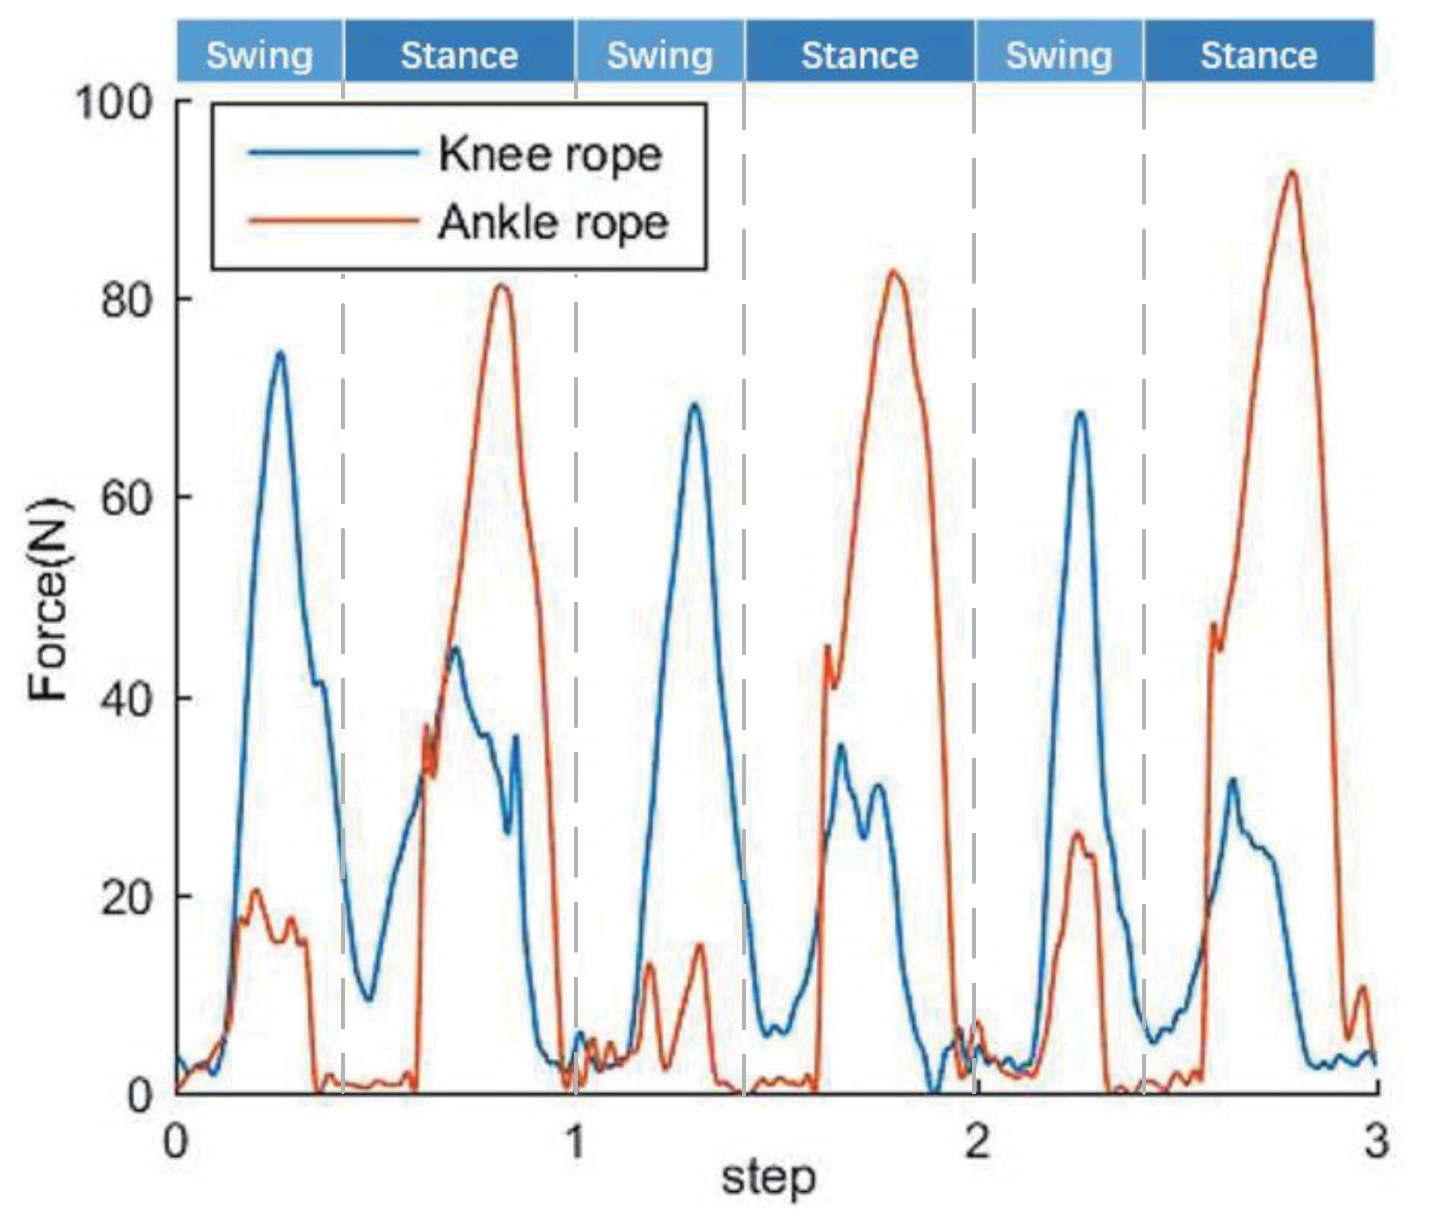
\includegraphics[width=8.5cm]{forces.eps}
	\caption{The forces in the knee rope (blue line) and ankle rope (orange line) in three typical gait cycles.}
	\label{fig:force}
\end{figure}

\subsubsection{Forces in the Ropes}
The functionality of the mechanical and control systems is verified by the recorded forces in both ropes.
The forces in three typical gait cycles of an exoskeleton wearer are depicted in Fig. \ref{fig:force}.
The average peak force in the knee rope (blue line) was 55$\pm$6 N, indicating the spring was stretched by the knee joint, and therefore some energy was stored in the torsion spring in late swing.
The average peak force in the ankle rope (orange line) was 73$\pm$5 N.
It can be clearly seen that the force increasing pattern in the ankle rope can be divided into two stages by different slopes during mid-stance phase.
In the first stage, a sharp increase indicates that the stretched spring (by the knee joint) began to exert force at the ankle, which led to a sudden change in the force.
In the second stage, the slope became milder, indicating the spring was stretched again by the ankle and began to store energy.
This result demonstrates the energy is properly recycled and released by the torsion spring as designed.

\begin{figure*}[t]
	\centering
	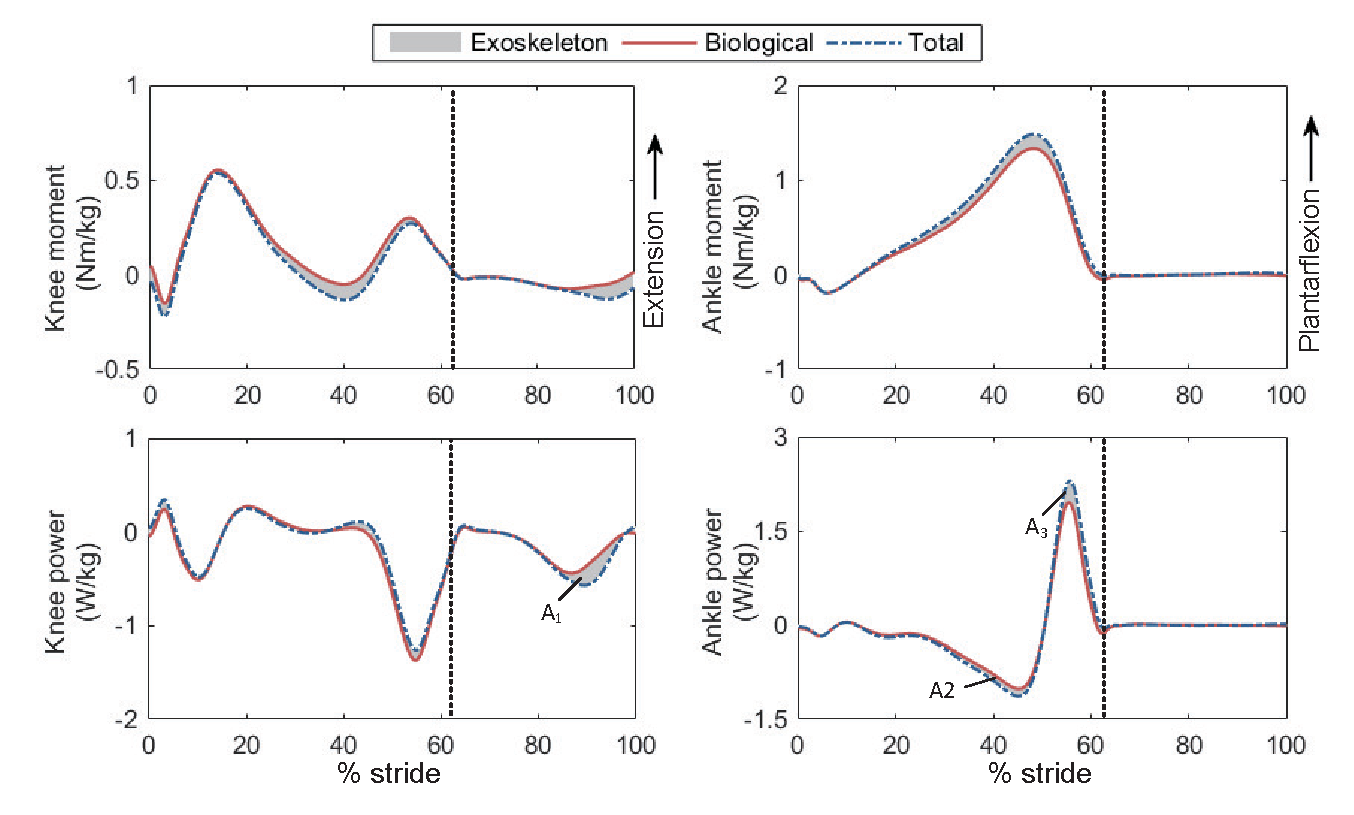
\includegraphics[width=17cm]{exo.eps}
	\caption{The moments and power of knee and ankle joints in the EXO\_ON condition.
	The total and biological data are shown in blue dash-dot and red solid lines, respectively.
	The shaded areas represent the moments and power provided by the quasi-passive exoskeleton.
	Stance phase and swing phase are separated by the black dotted line.}
	\label{fig:exo}
\end{figure*}

\subsubsection{Changes in Kinematics}
Joint angles, biological moments and power in the three conditions of the right leg where the exoskeleton was worn are presented in Fig. \ref{fig:kinetics_r}.
The EXO\_ON, EXO\_OFF and NO\_EXO conditions correspond to the red solid, blue dot-dash and gray dashed lines, respectively.
The knee joint and hip joint angles over the whole stride for all three walking conditions had no significant differences.
The peak ankle dorsiflexion angle during the stance phase in the EXO\_ON condition ($11.6\pm2.5$ degrees) was significantly smaller than that in the EXO\_OFF condition ($15.7\pm3.8$ degrees, $p=0.0298$).
A possible explanation is that the exoskeleton supplied some energy recycled from the knee joint to assist ankle plantar flexion, which in turn lowered the necessary dorsiflexion angle for the ankle joint to store the needed energy.
In other words, the stretched spring (by the knee joint) applied a large moment at the ankle, which might prevent it achieving the normal dorsiflexion angle.

\begin{figure*}[th]
	\centering
	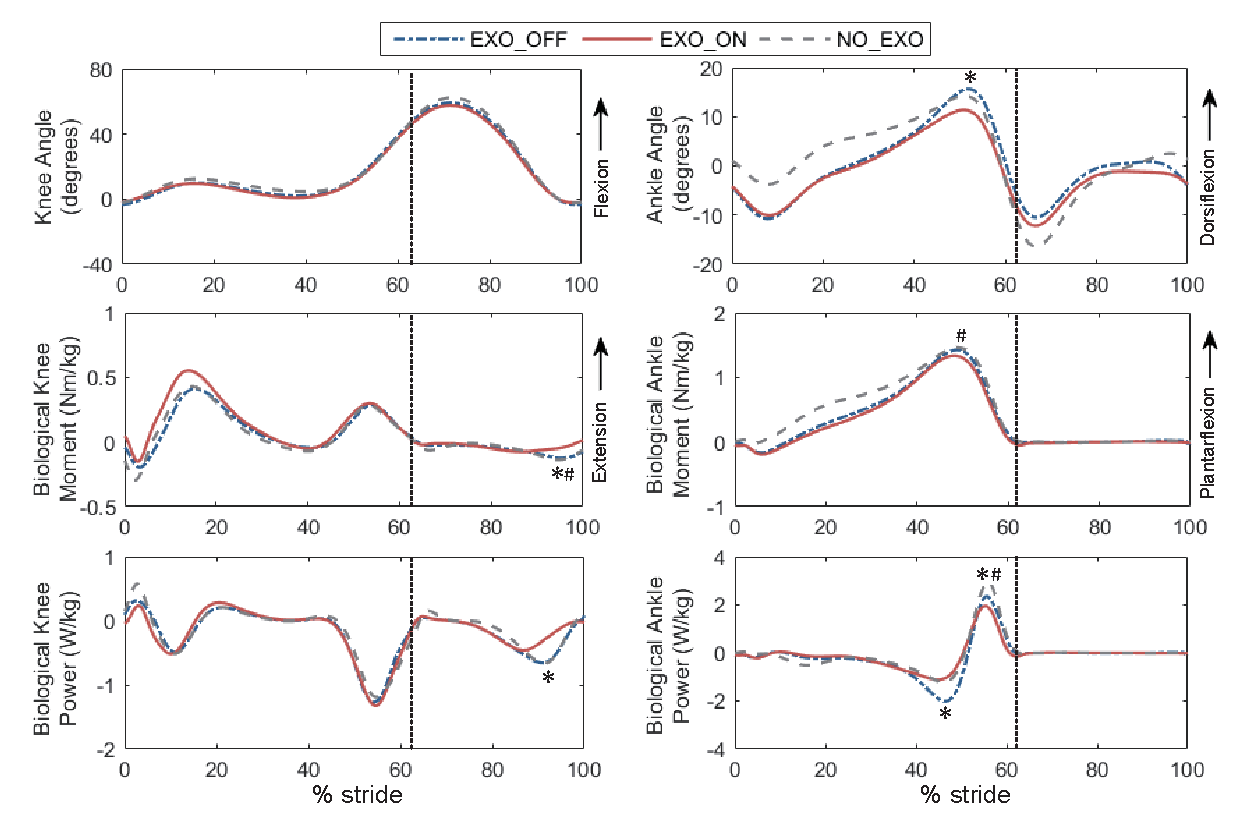
\includegraphics[width=17cm]{compare.eps}
	\caption{Right Leg Joint kinematics and kinetics.
		The joint angle, biological moment and power (from top to bottom) are shown for the ankle, knee and hip joints (from left to right) for the EXO\_ON (red solid line), EXO\_OFF (blue dash-dot line) and NO\_EXO (gray dashed line) conditions.
		The stance phase and swing phase are separated by black dotted lines.
		The markers $*$ and $\circ$ indicate significant differences ($p<0.05$) comparing the EXO\_ON condition to the EXO\_OFF condition and the NO\_EXO condition, respectively.}
	\label{fig:kinetics_r}
\end{figure*}

\subsubsection{Exoskeleton Power and Work}
For the EXO\_ON condition, the total (blue dash-dot), exoskeleton (shaded), and biological (red solid) joint moments and power averaged across eight subjects are shown in Fig. \ref{fig:exo}.

In late swing phase, the maximal moment and negative power of the exoskeleton applied to the knee joint were $0.093\pm0.017$ Nm/kg and $0.271\pm0.037$ W/kg respectively.
The negative work produced by the exoskeleton over late swing phase (80-100\% stride) was $1.43\pm0.36$ J (area A$_{1}$ in Fig. \ref{fig:exo}), accounting for 28\% of the total negative knee work during the same period.
This suggests the exoskeleton successfully recycled some negative work from the knee joint and assisted it in decelerating the shank.

In mid and late stance phases, the exoskeleton produced moments in the same direction as the biological ankle moments.
The maximal exoskeleton moment applied to the ankle joint was $0.156\pm0.013$ Nm/kg.
The maximal negative power of the exoskeleton during dorsiflexion was $0.126\pm0.029$ W/kg, and the maximal positive power during plantar flexion was $0.449\pm0.029$ W/kg.
The negative work produced by the exoskeleton to the ankle joint was $1.66\pm0.28$ J (area A$_{2}$ in Fig. \ref{fig:exo}), accounting for 13\% of the total negative ankle work (30\%-50\%).
The positive work produced by the exoskeleton was $2.39\pm0.35$ J (area A$_{3}$ in Fig. \ref{fig:exo}) , accounting for 20\% of the total positive ankle work (50\%-60\%).
These results suggest the exoskeleton is able to recycle some negative work from the ankle joint during mid-stance dorsiflexion, and assist it in push-off during late stance plantar flexion.
The ratio of the energy released at push-off to that recycled from the knee and ankle joints was about 77.34\%.

\subsubsection{Reductions in Biological Moment and Power}
The maximal knee flexion moment during late swing phase was significantly reduced by 42\% ($p = 0.0004$) and 34.6\% ($p = 0.0102$) when comparing the EXO\_ON ($0.083\pm0.017$ Nm/kg) to the NO\_EXO ($0.143\pm0.032$ Nm/kg) and EXO\_OFF conditions ($0.127\pm0.035$ Nm/kg) , respectively.
This reduction indicates that the exoskeleton provided considerable flexion moments and partially replaced muscles on the thigh to generate torques to decelerate the shank.
Furthermore, the biological negative knee work during the late swing phase had a significant reduction of 15.9\% ($p = 0.0138$) when comparing the EXO\_ON ($-0.061\pm0.016$ W/kg) to EXO\_OFF ($-0.073\pm0.022$ W/kg) conditions.
This reduced work seems to be recycled by the exoskeleton. However, the reduction from the NO\_EXO condition was not significant (p = 0.1875), which might indicate the negative effects of the extra weight introduced by the exoskeleton are still too large and counteract the assisting effects.
These reductions partly verified the expected outcome (i).

One of the most positive outcomes of the exoskeleton was the reduction of the plantar flexion moment at the ankle joint during mid and late stance phases.
Comparing the EXO\_ON condition ($1.347\pm0.096$ Nm/kg) to the NO\_EXO condition ($1.491\pm0.071$ Nm/kg), 9.6\% ($p = 0.0052$) significant reduction was reported, whereas the reduction was not significant in terms of the EXO\_OFF  condition ($p = 0.0876$).
The biological ankle negative work in the EXO\_ON condition ($0.193\pm0.046$ W/kg) during dorsiflexion was significantly decreased by 31.2\% ($p = 0.0089$) from the EXO\_OFF condition ($0.280\pm0.062$ W/kg) , whereas the reduction from the NO\_EXO condition was not significant ($p = 0.4086$).
These reductions might indicate reduced calf muscle forces due to the partial unloading of the Achilles’ tendon by the exoskeleton, and correspond to the expected outcome (ii).
During plantar flexion, the biological ankle positive power decreased significantly by 9.3\% ($p = 0.0027$) when comparing the EXO\_ON condition ($0.119\pm0.025$ W/kg) to the NO\_EXO condition ($0.131\pm0.028 W/kg$), and by 29.7\% ($p = 0.0201$) to the EXO\_OFF condition ($0.169\pm0.35$ W/kg).
From these reductions which verify expected outcome (iii), it can be concluded that the exoskeleton supplied the harvested energy to assist ankle plantar flexion in late stance.

\subsubsection{No Significant Change in the Hip or Left Leg}
The hip joint moment and power did not show any significant differences over the entire gait cycle.
As the exoskeleton is designed for assisting the knee and ankle joints, it was expected that the hip joint was not affected a lot by the exoskeleton.
In addition, the inverse kinematics and dynamics of the left leg where no exoskeleton was worn in the EXO\_ON and EXO\_OFF conditions were also calculated.
The average joint angles, moments and power which appeared different were tested, however, all of the differences were not significant among the three conditions for the left leg, thus the data are omitted here.
This might suggest the asymmetry of not wearing an exoskeleton on the left leg did not contribute a lot to the changes in kinematics and kinetics found in the right leg.

\subsubsection{Lost Energy due to Elastic Anchor}
A part of energy was lost because of the elastic anchor on the pants.
The exoskeleton produced a hindering torque on the knee joint in the stance phase, which can be observed from the force in the knee rope in Fig. \ref{fig:force}, as well as the increased biological moment and negative power at the knee joint from 40\% to 55\% of the gait cycle in Fig. \ref{fig:exo}. 
The maximal hindering torque produced by the exoskeleton was $0.083\pm0.024$ Nm/kg, and the corresponding maximal power was $0.177\pm0.069$ W/kg.

In normal walking, the knee joint undergoes slight flexion motions in stance, which causes the distance between the anchor on the thigh and the clutch-spring unit to decrease.
Since the pants were not entirely rigid even though some non-deformable safety belts were sewed into it, there were still some residue forces in the rope after the knee clutch locked.
As the knee flexed and extended, the residue force exerted a hindering moment at the knee joint, and some energy supposed to be recycled in the torsion spring was dissipated by the pants.
This is an inevitable side-effect for an elastic anchor, which might be reduced if a better fixation can be applied.
The flexible exoskeleton built by Lee \emph{et al.} \cite{exosuit} uses a unique support frame that withstands vertical loads while maintaining the natural curvature of the wearer's lower body, which could be used in future work.

\section{Conclusions and Future Work}
\label{sec:discussion}
In this paper, we present a quasi-passive lower limb exoskeleton which is able to recycle the negative work from the knee joint in late swing extension, and from the ankle joint in stance dorsiflexion to assist the ankle joint in push-off.
The major component of the exoskeleton is the clutch-spring unit which consists of a torsion spring as the energy storage element, and two actively controlled clutches attached at both ends of the spring to control the timings of recycling and releasing energy.
The novelty of this exoskeleton lies in the energy transferring mechanism from the knee joint to the ankle joint, which makes the dissipated energy in decelerating the shank reused to activate the velocity redirection of the COM through push-off.
Similar to a regenerative brake decelerating a hybrid car, this mechanism has the potential to make walking more efficient.

The functionality of the exoskeleton is verified by measuring the forces in the two ropes, which indicates the energy is properly recycled and released by the torsion spring controlled with the ratchets.
Inverse kinematics and dynamics analyses were performed on eight male subjects in three different walking conditions (NO\_EXO, EXO\_ON and EXO\_OFF).
Comparing the EXO\_ON to EXO\_OFF conditions, it can be seen that the biological moment and power were significantly reduced during the expected phases of movement (with the exception of the ankle moment in late stance phase).
This indicates the strategy of energy recycling and releasing is beneficial to human walking at joint level.
However, the extra weight and motion constraint introduced by the exoskeleton have a non-negligible effect on its uses.
This is indicated by the fact that a significant power reduction in the EXO\_ON condition compared with the NO\_EXO condition is seen only during push-off.

In future work, some efforts will be put into improving the mechanical and control systems.
Since the pressure sensors underfoot cannot provide any information in the swing phase, IMUs (Inertial Measurement Units) will be used to acquire the knee angle as an input to the control system \cite{IMU2,hao2019smoother}.
This will facilitate a better control on the timing to engage the knee clutch, which is now determined by a time delay after toe-off.
Also, the mechanical design of the clutch-spring unit will be optimized to make it lighter and smaller to alleviate the side-effect caused by the extra weight as seen in the experiment.
Round DC motors will replace the rectangular shaped servo motors to make the clutches more compact. 

Based on this described work, there are a number of follow-on human experiments that will be addressed in the future.
Specifically, lower limb muscle activities and metabolic expenditure during walking will be measured to evaluate the performance of the exoskeleton at physiological level, which will provide us with more details about how the exoskeleton interacts with human.

\begin{acknowledgment}
This work was supported in part by the National Key R\&D Program of China under Grant 2018YFC2001601, National Natural Science Foundation of China under Grant U1913205, U1613206 and 61533004, Guangdong Innovative and Entrepreneurial Research Team Program under Grant 2016ZT06G587, Shenzhen and Hong Kong Innovation Circle Project [Grant SGLH20180619172011638]; and Centers for Mechanical Engineering Research and Education at MIT and SUSTech.
\end{acknowledgment}
%%%%%%%%%%%%%%%%%%%%%%%%%%%%%%%%%%%%%%%%%%%%%%%%%%%%%%%%%%%%%%%%%%%%%%

% The bibliography is stored in an external database file
% in the BibTeX format (file_name.bib).  The bibliography is
% created by the following command and it will appear in this
% position in the document. You may, of course, create your
% own bibliography by using thebibliography environment as in
%
% \begin{thebibliography}{12}
% ...
% \bibitem{itemreference} D. E. Knudsen.
% {\em 1966 World Bnus Almanac.}
% {Permafrost Press, Novosibirsk.}
% ...
% \end{thebibliography}

% Here's where you specify the bibliography style file.
% The full file name for the bibliography style file 
% used for an ASME paper is asmems4.bst.
\bibliographystyle{asmems4}

% Here's where you specify the bibliography database file.
% The full file name of the bibliography database for this
% article is asme2e.bib. The name for your database is up
% to you.
%\bibliography{walking}
\bibliography{exoskeleton}

%%%%%%%%%%%%%%%%%%%%%%%%%%%%%%%%%%%%%%%%%%%%%%%%%%%%%%%%%%%%%%%%%%%%%%
\clearpage
\listoffigures
\clearpage
\listoftables
\end{document}
